\documentclass[conference]{IEEEtran}
\usepackage{times}
\usepackage{graphicx}

% numbers option provides compact numerical references in the text. 
\usepackage[numbers]{natbib}
\usepackage{multicol}
\usepackage[bookmarks=true]{hyperref}

\usepackage{comment}
\usepackage{xspace}
\let\labelindent\relax %fixes error in enumitem created due to legacy reasons
\usepackage{enumitem}
\usepackage{amsmath,amssymb,amsfonts,amsthm}
\usepackage{algorithm,algorithmicx}
\usepackage[noend]{algpseudocode}
\algrenewcommand\algorithmicindent{1em} 

\usepackage{parskip}
%\usepackage{subfig}
\usepackage{subcaption}
\usepackage[dvipsnames]{xcolor}

\DeclareMathOperator*{\argmin}{arg\,min}
%\pdfinfo{
%   /Author (Homer Simpson)
%   /Title  (Robots: Our new overlords)
%   /CreationDate (D:20101201120000)
%   /Subject (Robots)
%   /Keywords (Robots;Overlords)
%}


\graphicspath{
	{./figs/}
}

\hypersetup{letterpaper,bookmarksopen,bookmarksnumbered,
pdfpagemode=UseOutlines,
colorlinks=true,
linkcolor=blue,
anchorcolor=blue,
citecolor=blue,
filecolor=blue,
menucolor=blue,
urlcolor=blue
}

% Caligraphic letters:
\newcommand{\calA}{\ensuremath{\mathcal{A}}\xspace}
\newcommand{\calC}{\ensuremath{\mathcal{C}}\xspace}
\newcommand{\calE}{\ensuremath{\mathcal{E}}\xspace}
\newcommand{\calG}{\ensuremath{\mathcal{G}}\xspace}
\newcommand{\calR}{\ensuremath{\mathcal{R}}\xspace}
\newcommand{\calM}{\ensuremath{\mathcal{M}}\xspace}
\newcommand{\calN}{\ensuremath{\mathcal{N}}\xspace}
\newcommand{\calX}{\ensuremath{\mathcal{X}}\xspace}
\newcommand{\calS}{\ensuremath{\mathcal{S}}\xspace}
\newcommand{\calQ}{\ensuremath{\mathcal{Q}}\xspace}
\newcommand{\calT}{\ensuremath{\mathcal{T}}\xspace}
\newcommand{\calL}{\ensuremath{\mathcal{L}}\xspace}
\newcommand{\calB}{\ensuremath{\mathcal{B}}\xspace}
\newcommand{\calW}{\ensuremath{\mathcal{W}}\xspace}
\newcommand{\calV}{\ensuremath{\mathcal{V}}\xspace}
\newcommand{\calP}{\ensuremath{\mathcal{P}}\xspace}
\newcommand{\calD}{\ensuremath{\mathcal{D}}\xspace}
\newcommand{\calF}{\ensuremath{\mathcal{F}}\xspace}
\newcommand{\calO}{\ensuremath{\mathcal{O}}\xspace}


% math
\newcommand{\R}{\mathbb{R}}
\newcommand{\Z}{\mathbb{Z}}
\newcommand{\A}{\mathbb{A}}
\newcommand{\N}{\mathbb{N}}
\newcommand{\Q}{\mathbb{Q}}
\newcommand{\C}{\mathbb{C}}
\newcommand{\K}{\mathbb{K}}

% Motion planning
\newcommand{\Cfree}{\ensuremath{\calX_{\rm free}}\xspace}
\newcommand{\Cforb}{\ensuremath{\calX_{\rm forb}}\xspace}
%\newcommand{\Csafe}{\ensuremath{\calX_{\rm free}^{\rm safe}}\xspace}
\newcommand{\Cspace}{\calC-space\xspace}

% =
\newcommand{\eg}{{e.g.,}\xspace}
\newcommand{\ie}{{i.e.,}\xspace}
\newcommand{\etc}{{etc.}\xspace}
\newcommand{\etal}{{et~al.}\xspace}

\def\naive{{na\"{\i}ve}\xspace}

\def\OS#1{\textcolor{magenta}{#1}}
\def\FI#1{\textcolor{cyan}{#1}}

\newtheorem{thm}{Theorem}
\newtheorem{lem}{Lemma}
%\newtheorem{thm}{Theorem}[section]
\newtheorem{observation}[thm]{Observation}
%\newtheorem{thm}{Theorem}
\newtheorem{cor}{Corollary}
\newtheorem{definition}[thm]{Definition}


%tex tools
\newcommand{\ignore}[1]{}
\newcommand{\first}[2]{#1}
\newcommand{\second}[2]{#2}
\newcommand{\arxiv}[2]{#2}


\newcommand\algname[1]{\textsf{#1}\xspace}
\newcommand\astar{\algname{A*}}


%paper-related macros
\newcommand\Gfull{\ensuremath{G^{\textrm{full}}}\xspace}
\newcommand\Shome{\ensuremath{s_{\textrm{home}}}\xspace}
\newcommand\Tbound{\ensuremath{t_{\textrm{bound}}}\xspace}
\newcommand\Trc{\ensuremath{t_{\textrm{rc}}}\xspace}
\newcommand\Ssc{\ensuremath{s_{\textrm{sc}}}\xspace}


%comments
\def\os#1{\textcolor{magenta}{#1}}
\begin{document}

% paper title
\title{Provably Constant-time Planning and Re-planning for Real time Grasping Objects off a Conveyor}

% You will get a Paper-ID when submitting a pdf file to the conference system
\author{Author Names Omitted for Anonymous Review. Paper-ID [add your ID here]}

%\author{\authorblockN{Michael Shell}
%\authorblockA{School of Electrical and\\Computer Engineering\\
%Georgia Institute of Technology\\
%Atlanta, Georgia 30332--0250\\
%Email: mshell@ece.gatech.edu}
%\and
%\authorblockN{Homer Simpson}
%\authorblockA{Twentieth Century Fox\\
%Springfield, USA\\
%Email: homer@thesimpsons.com}
%\and
%\authorblockN{James Kirk\\ and Montgomery Scott}
%\authorblockA{Starfleet Academy\\
%San Francisco, California 96678-2391\\
%Telephone: (800) 555--1212\\
%Fax: (888) 555--1212}}


% avoiding spaces at the end of the author lines is not a problem with
% conference papers because we don't use \thanks or \IEEEmembership


% for over three affiliations, or if they all won't fit within the width
% of the page, use this alternative format:
% 
%\author{\authorblockN{Michael Shell\authorrefmark{1},
%Homer Simpson\authorrefmark{2},
%James Kirk\authorrefmark{3}, 
%Montgomery Scott\authorrefmark{3} and
%Eldon Tyrell\authorrefmark{4}}
%\authorblockA{\authorrefmark{1}School of Electrical and Computer Engineering\\
%Georgia Institute of Technology,
%Atlanta, Georgia 30332--0250\\ Email: mshell@ece.gatech.edu}
%\authorblockA{\authorrefmark{2}Twentieth Century Fox, Springfield, USA\\
%Email: homer@thesimpsons.com}
%\authorblockA{\authorrefmark{3}Starfleet Academy, San Francisco, California 96678-2391\\
%Telephone: (800) 555--1212, Fax: (888) 555--1212}
%\authorblockA{\authorrefmark{4}Tyrell Inc., 123 Replicant Street, Los Angeles, California 90210--4321}}


\maketitle

% \begin{abstract}
% Robots in warehouse environments typically perform repetitive tasks such as picking and placing of moving objects on a conveyor belt. Motion planning needs to be efficient and reliable in these domains to ensure high and consistent throughput. The success of manipulation tasks relies heavily on the accuracy of the perception system which often is noisy, especially if the target objects are perceived from a distance. For fast moving conveyor belts, the robot must start moving early on (relying on the first noisy estimate) to be able to reach the object in time and then adjust its motion as it gets improved estimates.
% To this end we propose a real-time replanning framework that would guarantee a bound on the reaction time of the robot whenever a perception update is received. Our key insight is that for repetitive tasks the paths look very similar and can efficiently be reused to minimise the processing time and memory footprint. Our framework leverages offline preprocessing to compute a representative set of paths (with some auxiliary data structures) which can then be used online to generate a plan from any point during execution (if one exists) in bounded time. We show our results on a 7 DOF robot arm, demonstrating the robot picking up objects from a conveyor belt.
% \end{abstract}

\begin{abstract}
In warehousing and manufacturing environments, manipulation platforms are excessively deployed on  conveyor belts to perform fast pick and place tasks. Because objects on the conveyor belts are moving,  robots have limited time to pick them up. This brings the need for fast and reliable motion planners that could provide constant-time planning guarantees. Besides the planning efficiency, the success of manipulation tasks relies heavily on the accuracy of the perception system which often is noisy, especially if the target objects are perceived from a distance. For fast moving conveyor belts, the robot cannot wait for a perfect estimate before it starts execution; it must start moving early on (relying on the initial noisy estimates) and adjust its motion on-the-fly to be able to reach the object in time. We propose an approach that meets these requirements by providing provable constant-time planning and replanning guarantees. We present it, give its analytical properties and show experimental analysis in simulation and on a real robot.
\end{abstract}


\IEEEpeerreviewmaketitle

\section{Introduction}
%1. What is the problem?
%2. Why is it relevant?
%3. Why is it hard?
%4. What have others done?
%5. What's missing?
%6. What is our ONE key insight?
%7. How do we compare against the state of the art?
%8. What are our contributions?
%9. What are our limitations?

%% motivation
Conveyor belts are widely used in automated distribution, warehousing, as well as for manufacturing and production facilities. In the modern times robotic manipulators are being deployed extensively on the conveyor belts for automation and faster operations [\os{add citations}]. In order to maintain a high distribution throughput, manipulators must pick up moving objects without having to stop the conveyor for every grasp. In this work, we consider the problem of motion planning for grasping moving objects off a conveyor. An object in motion imposes a requirement that it should be picked up in a short window of time. The motion planner for the arm, therefore, must compute a path within a bounded time frame to be able to successfully perform this task.

%% why replanning?
Manipulation relies on good quality detection and localization of moving objects. When the object first enters the field of view of the robot, the initial perception estimates of the object's pose are often inaccurate. Consider the example of an object (sugar box) moving along the conveyor towards the robot in Figure \ref{fig:pose_sequence}, shown through an image sequence as captured by the robot's Kinect camera. The black color denotes points corresponding to the object in the observed scene after filtering out all points lying outside the conveyor. The white point cloud shows the object's 3D model transformed with the predicted 3-Degree of Freedom pose obtained by using Iterative Closest Point (ICP) [\os{add citations}] refinement. Upon observation of the overlap between the point clouds, we see that they begin to overlap more closely as the object moves towards the robot, indicating that the pose estimate is becoming increasingly accurate. However, if the robot waits too long to get an accurate estimate of the object pose, the delay in starting plan execution could cause the robot to miss the object. The likelihood of this occurring increases proportionately with the speed of the conveyor. Therefore, the robot should start executing a plan computed for the initial pose and as it gets better estimates, repeatedly replan for the new goals. However, for every replanning query, the time window for the pickup shrinks and thus the motion planner must support real-time replanning.

\begin{figure}
    \centering
    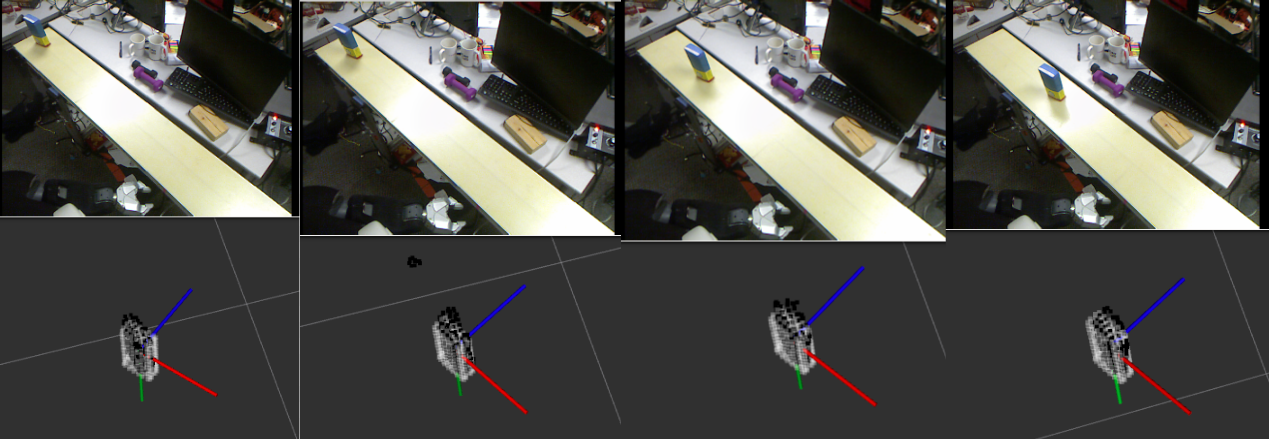
\includegraphics[width=0.5\textwidth]{figs/pose_sequence.png}
    \caption{\textit{Top} : Image sequence of a moving sugar box captured at 4 points along the conveyor. \textit{Bottom} : The observed points corresponding to the object (black) and the points corresponding to the object model transformed with the predicted pose (white).}
    \label{fig:pose_sequence}
\end{figure}
%% why problem is hard
The planning problem is challenging because the motion planner has to account for the dynamic object and thus plan in the time dimension. It should generate a valid trajectory that not only avoids collision with the environment around it but also with the target object to ensure that it does not damage or topple it during the grasp. Avoiding collisions with the object, requires precise geometric collision checking between the object geometry and the geometry of the manipulator's gripper links. The resulting complexity of the planning problem makes it infeasible to plan online for this task.

%%
We propose a planning framework that leverages offline preprocessing to provide bounds on the planning time when the planner is invoked online. Our key insight is that in our domain the manipulation task is highly repetitive---even for different object poses the computed paths are very similar and can be efficiently reused to speed up online planning. We precompute a representative set of paths offline with some auxiliary datastructures that can be used online to plan in constant time. For this work we assume that the models of the target objects are known. Namely, the planner will be provided with the geometric model of the target object apriori. To the best of our knowledge, non of the existing methods provides constant-time planning guarantees even for known environments. 

%
We experimentally show that constant-time planning and replanning capability is necessary for a successful conveyor pickup task. With one time planning, either following the plan for the initial noisy pose estimate or from a delayed but accurate pose estimate, both result in frequent failures.

\section{Related work}
\subsection{Motion Planning for Conveyor Pickup Task}
The existing work on picking up moving objects have been focused on different aspects of the problem ranging from closed loop controls to object perception and pose estimation, motion planning and others~\cite{allen1993automated, zhang2018gilbreth, stogl2017tracking, han2019toward} . For the sake of our discussion we will focus on motion planning related work. Graph-searched based approaches have been used for the motion planning problem~\cite{menon2014motion, cowley2013perception}. The former uses a kinodynamic motion planner to smoothly pick up moving objects i.e. without an impactful contact. They used a heuristic search-based motion planner that plans with dynamics and could generate optimal trajectories with respect to the time of execution. While their planner provides strong optimality guarantees, it is not real-time and thus cannot be used online.
%
The latter demonstrated their approach in the real world showing real-time planning capability. While their planner is fast, they do pure kinematic planning and they don't required collision checking with the target object. They plan to a pregrasp pose and rely on cartesian space controllers to perform the pick up. The usage of the cartesian controller limits the types of objects that the robot can grasp.

\subsection{Preprocessing-based Planning}
Preprocessing-based motion planners prove beneficial for real-time planning. They analyse the configuration space offline to generate some auxiliary information that can be used online to speed up planning. Probablistic RoadMaps (PRMs)~\cite{kavraki1996probabilistic} precomputes a roadmap that can answer any query by connecting the start and goal configurations to the roadmap and then searching the roadmap. PRMs are fast to query yet they do not provide constant time guarantees.
Moreover for the moving object, they would require edge re-evaluation which could be expensive.
%
A provably constant time planner was recently proposed~\cite{islam2019planning}. Given a start state and a goal region, it precomputes a compressed set of paths that can be utilised online to plan to any goal state within the goal region in bounded time. Our approach bears close resemblance with this work in the context of paths compression mechanism.
The vanilla versions of both of these approaches are only applicable to pure kinematic planning and thus they cannot be used for the conveyor planning problem.
%
Another family of preprocessing-based planners utilises previous experiences to speed up the search~\cite{PCCL12,BAG12,CSMOC15}. Experience graphs~\cite{PCCL12}, provide speed up planning times for repetitive tasks by trying to reuse previous experiences. These methods are also augmented with sparsification technques (see e.g.,~\cite{SSAH14,DB14}) to reduce the memory footprint of the algorithm.
Unfortunately, none of the mentioned algorithms provide bounded planning-time guarantees that are required by our application.

\subsection{Online Replanning}
The conveyor planning problem can be modelled as a Moving Target Search problem (MTS) which is a widely studied topic in the graph search-based planning literature~\cite{ishida1991moving,ishida1995moving,koenig2007speeding,koenig2007speeding,sun2010moving}. 
They interleave planning and execution incremently update the heuristic values of the state space to improve the distance estimates to the moving target. In higher dimensional planning problems, this process is expensive and this is why these approaches are typically used for 2d grid problem e.g for video games.



\section{Problem definition}
Our system is comprised of 
a robot manipulator $\calR$,
a conveyor belt moving $\calB$ moving at some known velocity,
a set of known objects $\calO$ that need to be grasped and 
a perception system $\calP$ that is able to estimate the type of object and its location on~$\calB$.

Given a pose $g$ of an object $o \in \calO$, our task is to plan the motion of $\calR$ such that it will be able to pick~$o$ from~$\calB$ at some future time.
%
Unfortunately, the perception system $\calP$ may give inaccurate object poses.
Thus, the pose $g$ will be updated by~$\calP$ as the robot is executing its motion. 
To allow for $\calR$ to move towards the updated pose in real time, we introduce the additional requirement that planning should be done within a predefined time bound~\Tbound.
%
For ease of exposition, when we say that we plan to a pose $g$ of $o$ that is given by $\calP$, 
we mean that we plan the motion of $\calR$ such that it will be able to pick~$o$ from~$\calB$ at some future time. 

%
We denote by $\Gfull$ the discrete set of configurations corresponding to the set of all possible initial object poses on $\calB$ that $\calP$ can perceive.
%
Finally, we assume that $\calR$ has an initial pose \Shome from which it will start its motion to grasp an object.
\os{add figure of conveyor belt}.

Roughly speaking, the objective, following the set of assumptions we will shortly state, is to enable planning to any goal pose $ g \in \Gfull$ in bounded time~\Tbound regardless of where the robot is currently placed.
%More specifically, the perception system is setup such that it sends updated pose estimates on the fly as the object moves along the conveyor belt and as the robot approaches the object.   
To formalize this idea, let us introduce the notion of a \emph{covered} state:
\begin{definition}
    A goal state $g \in \Gfull$ is said to be \emph{covered} by a state $s$ if 
    the system can plan a path from $s$ to $g$ within time~\Tbound.
\end{definition}

Thus, we wish to build a system such that 
for any state $s$ that the system can be in 
and every goal pose $g \in \Gfull$ updated by~$\calP$,
$g$ is covered by $s$.

We are now ready to state the assumptions for which we can solve the problem defined.

\begin{definition}
    A goal state $g \in \Gfull$ is said to be \emph{reachable} from a state $s$ if there exists a path from $s$ to $g$ and it can be computed in finite time.
\end{definition}

Given a state $s$ we denote the set of all goal states that are reachable from $s$ as $G^{\rm reach}(s)$ and we say that $G^{\rm reach}(s)$ is \emph{reachable} from $s$.


%\begin{definition}
%    A goal region $G \subseteq \Gfull$ is said to be \emph{reachable} from a state $s$ if any state $g \in G$ is reachable from $s$.
%\end{definition}

We make the following assumptions about the system.
\begin{enumerate}[label={\textbf{A\arabic*}},leftmargin=0.75cm]
    \item \label{assum:1} The goal set \Gfull is reachable from the start state~\Shome. Namely,  $G^{\rm reach}(\Shome) = \Gfull$.
    
\ignore{
    \item \label{assum:2} Given a path 
    $\Pi = \{s_0, \ldots, s_k \}$ 
    s.t. $s_0 = \Shome$ and $s_k \in \Gfull$, 
    we have that $G^{\rm reach}(s_{i+1}) \subset G^{\rm reach}(s_{i})$.
    Namely, the reachable set of goals for a state on the path is a subset of the reachable set of every other state on that path that exists before it.
    \os{Oren - Didn't we agree that this is not an assumption but a property?}
}

%    \item \label{assum:3} \Gfull would accommodate for an error $\epsilon$ in the initial pose estimate $g_{\textrm{init}}$ of the perception system. Each subsequent estimate $g_{\textrm{next}}$ will be within the $\epsilon$ window around $g_{\textrm{init}}$ (in retrospect because the conveyor is moving).
 
    \item \label{assum:3} Given an initial pose estimation $g_{\textrm{init}} \in \Gfull$ by $\calP$, any subsequent estimation $g_{\textrm{new}} \in \Gfull$ is at most $\varepsilon_\calP$ distance away from $g_{\textrm{init}}$ (after accounting for the fact that the object moved along $\calB$).

    \item \label{assum:4} There exists a replan cutoff time \Trc from when the robot starts moving, after which the perception system does not update the object's pose.
    
    \item \label{assum:5} If the robot starts moving at $t = 0$ then for any time $t < \Trc$, the environment is static. Namely, objects on~$\calB$ cannot collide with $\calR$ during that time.
\end{enumerate}

Assumption~\ref{assum:1} corresponds to properties of the environment \emph{without} taking the objects on the conveyor belt into account 
while
Assumptions~\ref{assum:3}-\ref{assum:5} correspond to properties of the environment that account for the perception system and the objects on the conveyor belt.


\section{Algorithmic framework}
\label{subsec:strawman}
Our approach for bounded-time planning relies on a \emph{preprocessing} stage that allows to efficiently compute paths in a \emph{query} stage to any goal state (under Assumptions~\ref{assum:1}-\ref{assum:5}). 
%
Before we describe our approach, we start by describing a \naive method that solves the aforementioned problem but requires a prohibitive amount of memory.
%
This can be seen as a warmup before describing our algorithm which exhibits the same traits but doing so in a memory-efficient manner.

\subsection{Straw man approach}
We divide the preprocessing stage into two steps.
In the first step, we compute from \Shome a path $\Pi_g$ to every goal state $ g \in \Gfull$ (such a path exists following \ref{assum:1}).
Thus, all goal states are covered by \Shome and this allows us to start executing a path once $\calP$ gives its initial pose estimate.
However, we need to allow for updated pose estimations while executing a path~$\Pi_g$. 

%
Following \ref{assum:4} and \ref{assum:5}, this only needs to be done up until time~\Trc.
Thus. we discretize each path such that consecutive states along the path are no more than $\delta _t$ time apart. As we will see, this will allow the system to start executing a new path within $\Tbound + \delta_t$ after a new pose estimation is obtained from $\calP$.
%
We call all states that are less than \Trc time from \Shome \emph{replanable states}.


In the second step of the preprocessing stage, for every replanable state along each path $\Pi_g$, we compute a new path to all goal states \bound{that are $\varepsilon_\calP$ away from $g$}.
For a visualization, see Fig.~\ref{fig:naive}.
%
This will ensure that all goal states are covered by the replanabale states that were introduced in the first step of the preprocessing stage. Namely, it will allow to immediately start executing a new path once the goal location is updated by $\calP$.
%
Unfortunately, $\calP$ may update the goal location more than once. Thus, this process needs to be performed recursively for the new paths as well.


The outcome of the preprocessing stage is a set of precomputed collision-free paths starting at states that are at most $\Trc$ from \Shome and end at goal states.
The paths are stored in a lookup table that can be queried in $O(1) < \Tbound$ time.

In the query stage we obtain an estimation $g_1$ of the goal pose by $\calP$. 
The algorithm then retrieves the path~$\Pi_1(\Shome,g_1)$ from~\Shome to~$g_1$ and the robot starts executing~$\Pi_1(\Shome,g_1)$.
%
For every new estimation $g_i$ of the goal pose obtained from $\calP$  while the system is executing path $\Pi_{i-1}(s,g_{i-1})$, the algorithm retrieves from the lookup table the path $\Pi_i(s',g_i)$ from the first state~$s'$ along $\Pi_{i-1}(s,g_{i-1})$ that $\Tbound + \delta_t$ from~$s$ and the robot will then start executing~$\Pi_i(s,g_i)$ once it reaches~$s'$.

Clearly, every state is covered by this brute-force approach, however it requires a massive amount of memory.
Let $n_{\rm goal} = \vert \Gfull \vert$ be the number of goal states and
$\ell$ be the number of states between \Shome and the state that is \Trc time away.
This approach requires storing $O(n_{\rm goal}^\ell)$ paths which is clearly infeasible.
In the next sections, we show how we can dramatically reduce the memory footprint of the approach without compromising on the system's capabilities.



\begin{figure}[t]
    \centering
    \begin{subfigure}{.225\textwidth}
    %   \centering
        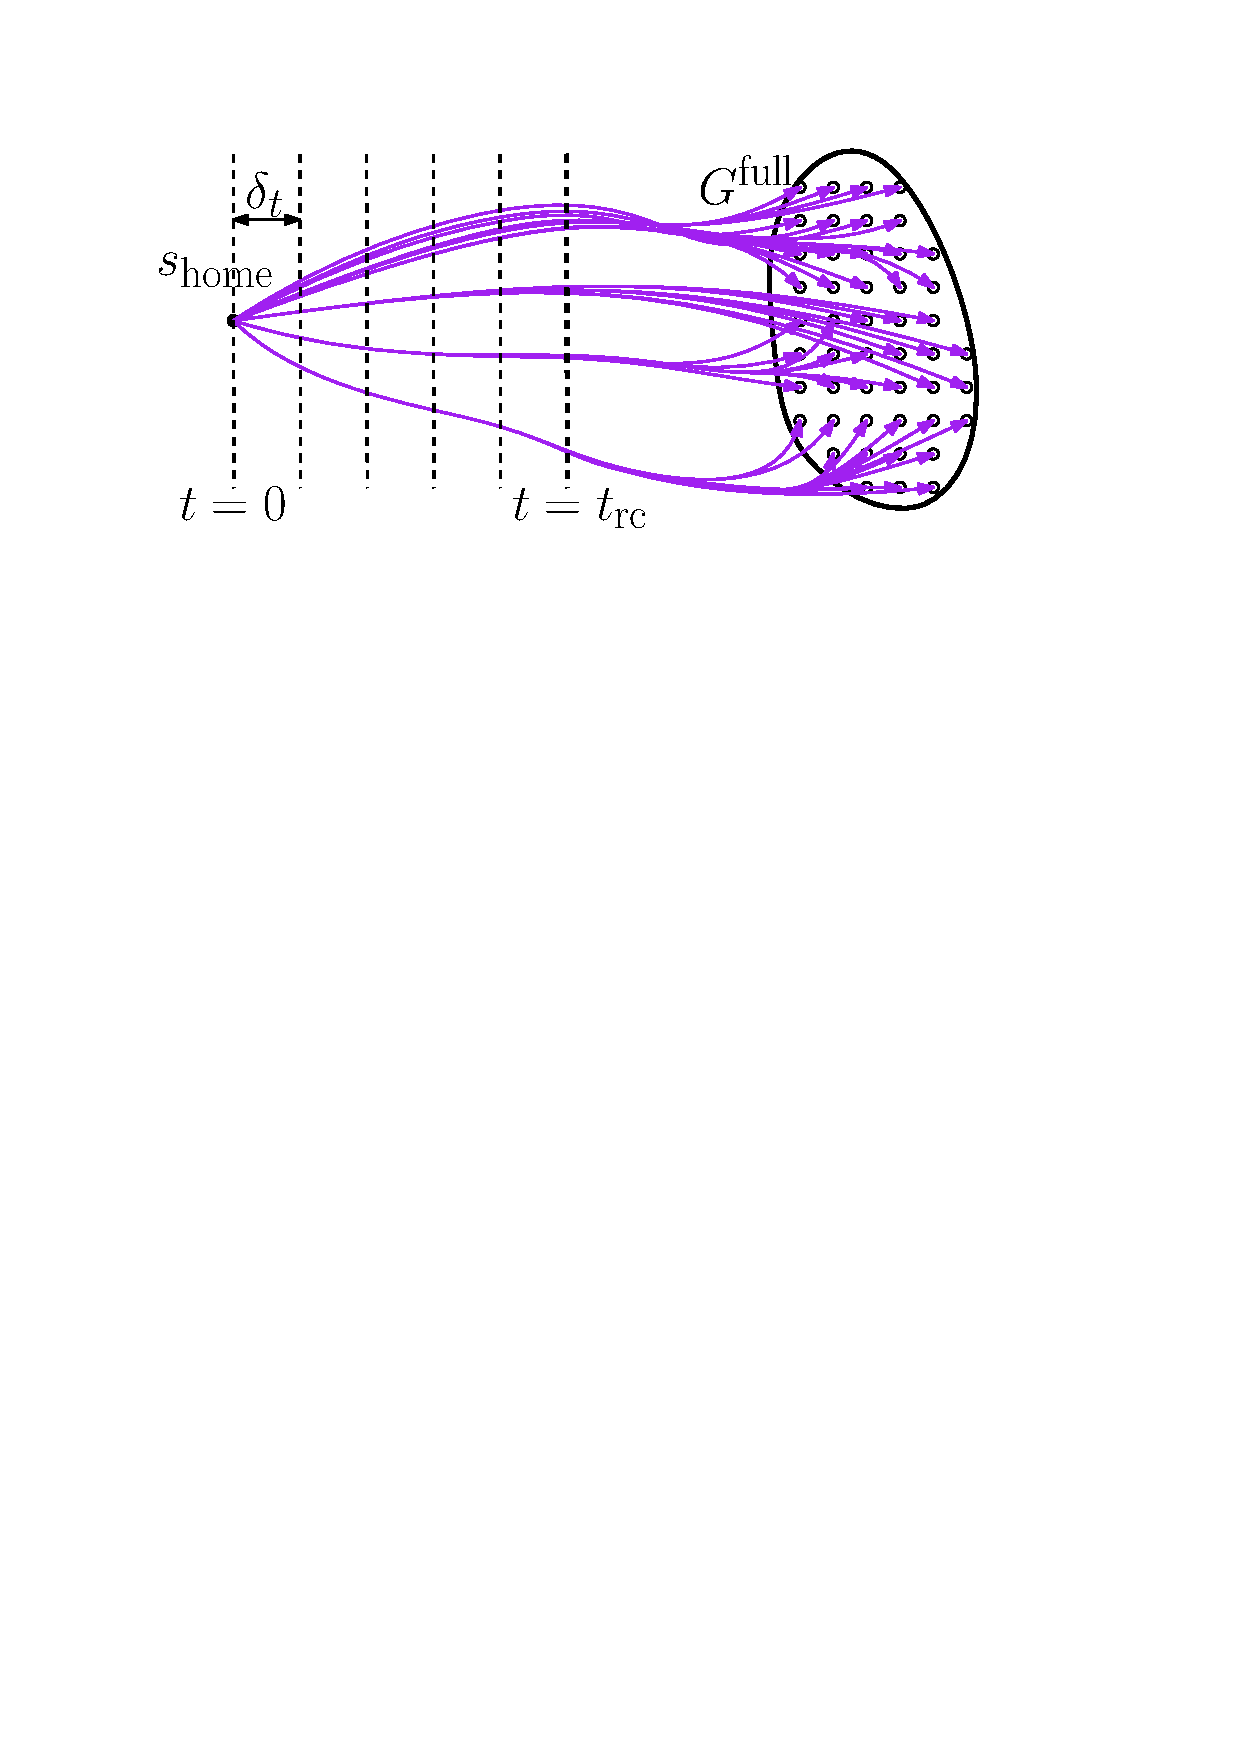
\includegraphics[width=\textwidth]{naive1}
        \caption{}
        \label{fig:naive1}
    \end{subfigure}
    \hfill
    \begin{subfigure}{0.225\textwidth}
    %   \centering
        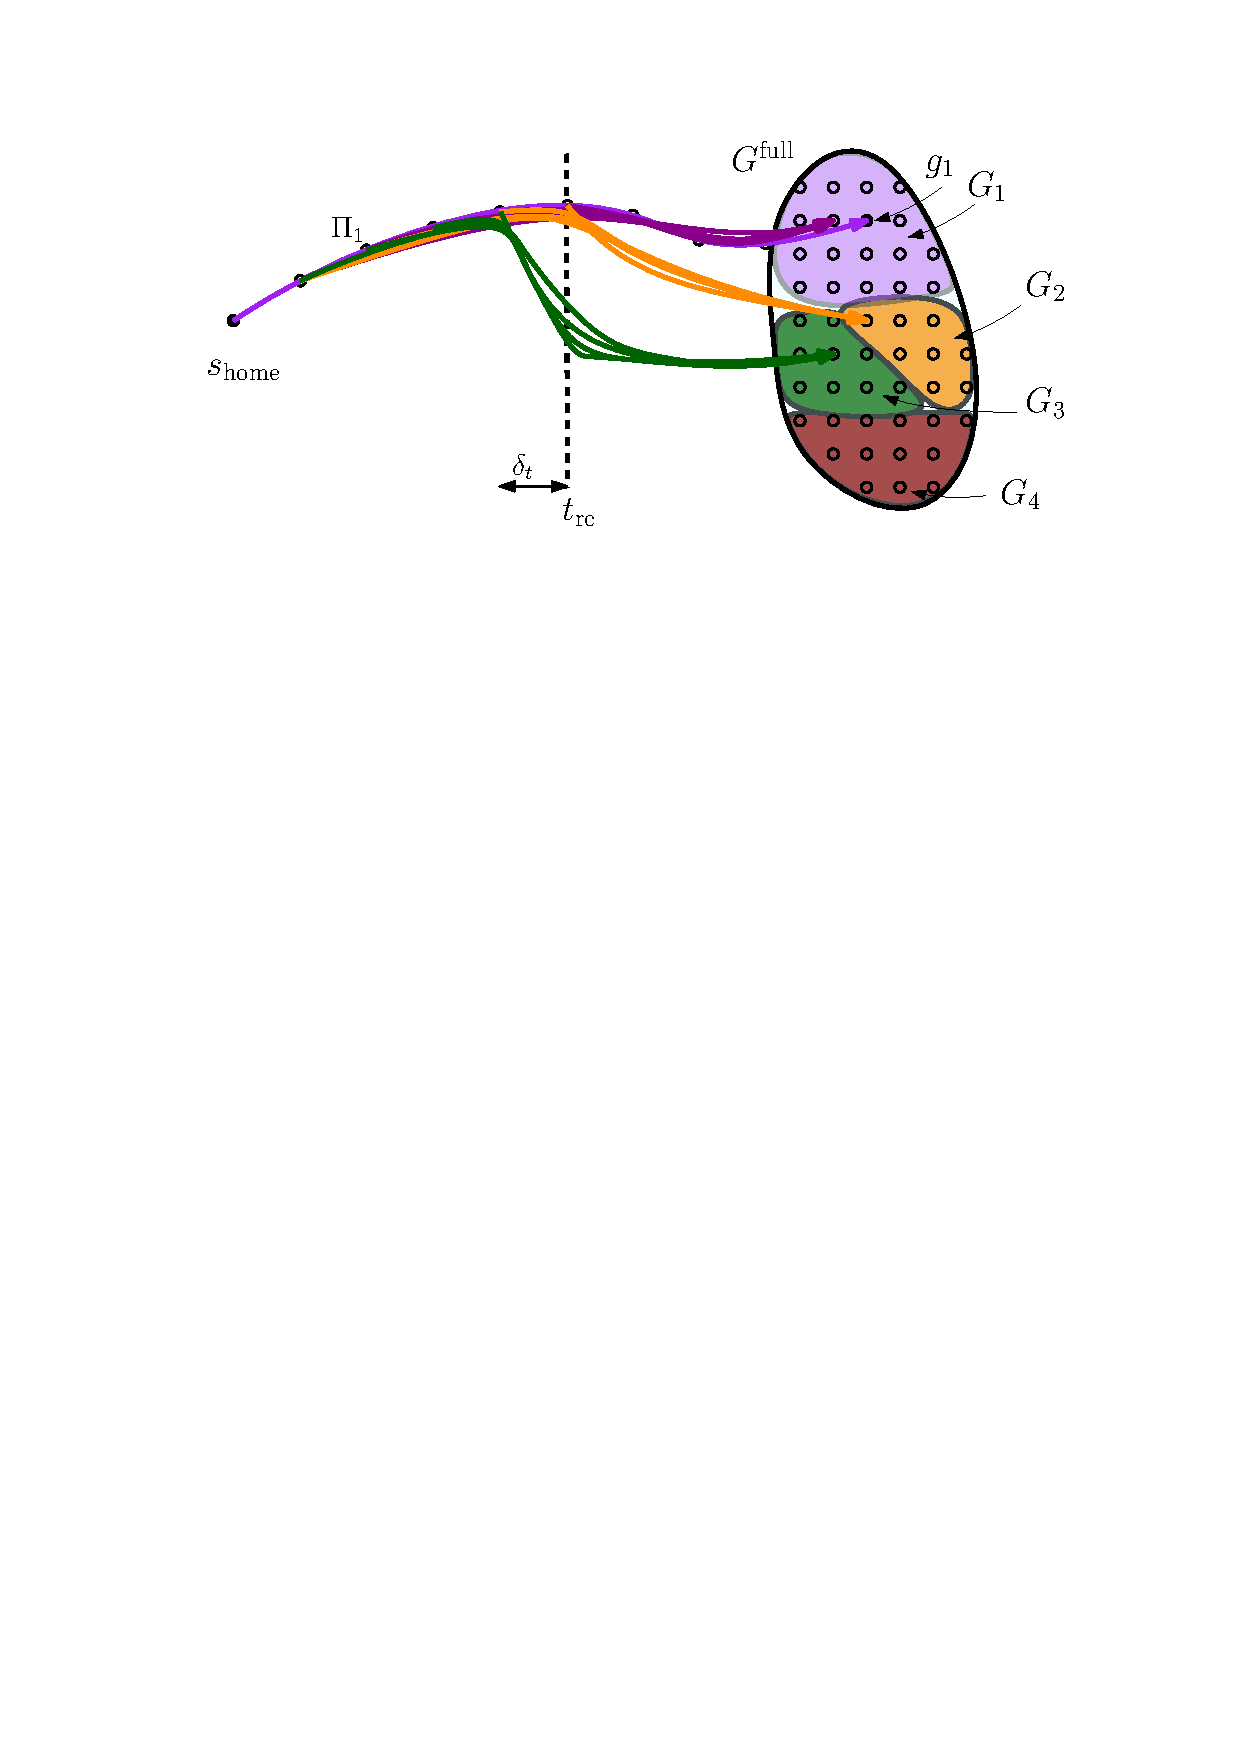
\includegraphics[width=\textwidth]{naive2}
        \caption{}
        \label{fig:naive2}
    \end{subfigure}
    \caption{The two steps of the preprocessing stage of the straw man algorithm. In both figures, paths that are very similar (and their corresponding goal states) are depicted using the same color.
    (\subref{fig:naive1})~First step---the algorithm computes a path from \Shome to every state in \Gfull.
    %
    (\subref{fig:naive2})~Second step---the algorithm computes for each path a new path to each goal state for every state along the path. Here, one representative path is depicted together with three different goal states. 
    This is repeated recursively for the new paths but not visualized.}
    \label{fig:naive}
\end{figure}

\subsection{Algorithmic approach}
While the straw man algorithm presented in Sec.~\ref{subsec:strawman} allows for planning to any goal pose $ g \in \Gfull$ in bounded time~\Tbound, its memory footprint is prohibitively large.
%
We suggest to reduce the memory footprint by building on the observation that many paths to close-by goals traverse very similar parts of the configurations space (see Fig.~\ref{fig:naive}).

Similar to the straw man algorithm, our preprocessing stage runs in two steps.
In the first step we we compute from \Shome a path $\Pi_g$ to every goal state $ g \in \Gfull$. However, this is done by computing a set of so-called ``root paths'' $\{\Pi_1, \ldots, \Pi_k \}$ from \Shome to a subset of goals in \Gfull (here we will have that $k \ll n_{\rm goal})$. 
As we will see, these paths will allow to efficiently compute paths to every goal state in the query stage and the system only needs to explicitly store these root paths in memory (and not a path to every goal state as in the straw man algorithm).
%
In the second step of the preprocessing stage, the algorithm recursively computes for all replanabale states along all root paths a new path to each goal state. However, this is done by attempting to re-use previously-computed root paths which, in turn, allows for a very low memory footprint.
%
It is important to note that replanable states are not only the ones that lie on the root paths from \Shome---whenever the recursion happens we compute a new set of root paths and generate new replanable states
%
The remainder of this section formalizes these ideas.

\subsection{Algorithmic building blocks}
We start by introducing the algorithmic building blocks that we use.
Specifically, we start by describing the motion planner that is used to compute the root paths 
and then continue to describe how they can be used as \emph{experiences} to efficiently compute paths to near-by goals.
\subsubsection{Motion planner}
We use a heuristic search-based planning approach with motion primitives~\cite{}
as it allows for deterministic planning time which is key in our domain.
Moreover, such planners can easily handle under-defined goals as we have in our setting---we define a goal as a six DoF grasp pose for the goal object while our robot has seven DoFs and we need to acount for the grasping time.

\textbf{State space and graph construction.}
We define a state $s$ as a pair $(q,t)$ where $q = (\theta_1, ..., \theta_n)$ is a configuration represented by the joint angles for an $n$-DOF robot arm (in our setting $n=7$)and $t$ is the time associated with $s$.
%
Given a state $s$ we define two types of motion primitives which are short kinodynamically feasible motions that the robot~$\calR$ can execute. The first, which we term \emph{predefined} primitives are used to move a pre-grasp position while the second, termed \emph{dynamic} primitives are used to perform grasping after the robot reached a pre-grasp position.
%
The predefined primitives are small individual joint movements in either direction as well as wait actions.
For each motion primitive, we compute its duration by using a nominal constant velocity profile for the  joint that is moved.\footnote{Computing a plan using these motion primitives is not guaranteed to respect the acceleration limits of $\calR$. However, in practice this seldom occurs and we elaborate in Sec.~\ref{sec:eval} how we handle these execution errors.}.
%
The dynamic primitives are generated by using a Jacobian pseudo inverse-based control law. 
The velocity of the end effector is computed such that the end-effector minimises distance to the grasp pose. Once the gripper encloses the object, it moves along with the object until the gripper is closed.
Additional details omitted due to lack of space.

\textbf{Motion planner.}
The states and the transitions implicitly define a graph $\calG = (S,E)$ where $S$ is the set of all states and $E$ is the est of all transitions defined by the motion primitives. We use Weighted \astar (\wastar) to find a path from a given state $s$ to a goal $g$ states on $\calG$. 
\wastar is a suboptimal heursitic search that tradesoff optimality and greediness by inflating the heuristic function by a given weight $w$. 
The search is guided by an efficient and fast-to-compute heuristic function which in our case has two components.
The first component drives the search to intercept the object at the right time and 
the second component guides the search to correct the orientation of the end effector as it approaches the object. 
More formally, our heuristic function is given by
$$
 h(s,g) = \max (w \cdot t(s,g), \textsc{AngleDiff}(s,g)).
$$
Here, $t(s,g)$ is the expected time to intercept the object which can be analytically computed from the velocities and positions of the target object and the end-effector and \textsc{AngleDiff}($s,g$) gives the the magnitude of angular difference between the end-effector's current pose and target pose.

\subsubsection{Planning using experiences}
We now show how \emph{experience graphs}~\cite{PCCL12} can be used in our framework.
%
Roughly speaking, experience graphs allow a planner  to accelerate its planning efforts whenever possible by using previously-computed paths. The planner gracefully degenerates to planning from scratch if no previous planning experiences can be reused.
%
The key idea is to bias the search efforts, using a specially-constructed heuristic function (called the ``e-graph heuristic''), towards finding a way to get onto the previously-computed paths and to remain on them rather than explore new regions as much as possible. 

In our setting, we use a simplified version of the aforementioned approach which is faster to compute.
%
The key insight is that in our setting, we always start at \Shome which is the first state on all root paths. Thus, we only need to bias the search to stay on a root path (and we don't need to bias the search efforts to get onto the previously-computed paths).
%
To this end, given a heuristic function $h$ we define for each root path $\Pi$ and each goal state $g \in \Gfull$ the \emph{shortcut} state $\Ssc (\Pi,g)$ as the   state that is closest to~$g$ with respect~$h$.
Namely,
$$
\Ssc (\Pi,g) := \argmin\limits_{s_i \in \Pi} h(s_i, g).
$$
Now, when searching for a path to a goal state $g \in \Gfull$ we
(i)~add $\Ssc (\Pi,g)$ as a successor for any state along $\Pi$
(subject to the constraint that the path along $\Pi$ to \Ssc is collision free)
and
(ii)~update our heuristic function to bias the search to use root paths. Specifically, for any state $s$ on the root path $\Pi$ the heuristic is given by
$$
h(s,g) = \min(h(s,\Ssc (\Pi,g)) + h(\Ssc (\Pi,g),g), \varepsilon \cdot h(s,g)).
$$
Here, $\varepsilon>1$ is a penalty term that biases the search to find a path via \Ssc.

\os{We will probably get rid of this heuristic function}

\fis {Oren - We should either use the term experience or root path throughout the paper}

\os{Fahad - I don't agree. Root paths are what we compute and they use experience graphs to speed up computation. E-graphs are the tool and root paths are they way we use the tool.}


\subsection{Algorithmic details}
\subsubsection{Preprocessing}
Our preproccesing stage starts by sampling a goal state $g_1 \in \Gfull$ and computing a root path $\Pi_1$ from $\Shome$ to $g_1$. We then associate with $\Pi_1$ all goal states $G_1 \subset \Gfull$ such that $\Pi_1$ can be used as an experience in reaching any state in $g_1' \in G_1$ 
Thus, all goal states in $G_1$ are covered by \Shome.
%
We then repeat this process but instead of sampling  a goal state from \Gfull, we sample from $\Gfull \setminus \Gcov$, where \Gcov is the set of goal states already covered by \Shome.
At the end of this step, we obtain a set of root paths. 
Each root path $\Pi_i$ is associated with a goal set $G_i \subseteq \Gfull$ such that 
(i)~$\Pi_i$ can be used as an experience in reaching any state in $g_i' \in G_i$ and 
(ii)~$\bigcup_i G_i = \Gfull$.
%
For a visualization of this step, see Fig.~\ref{fig:crp}.
For pseudocode see Alg.~\ref{alg:step1}.

\begin{figure*}[t]
    \centering
    \begin{subfigure}{.3\textwidth}
    %   \centering
        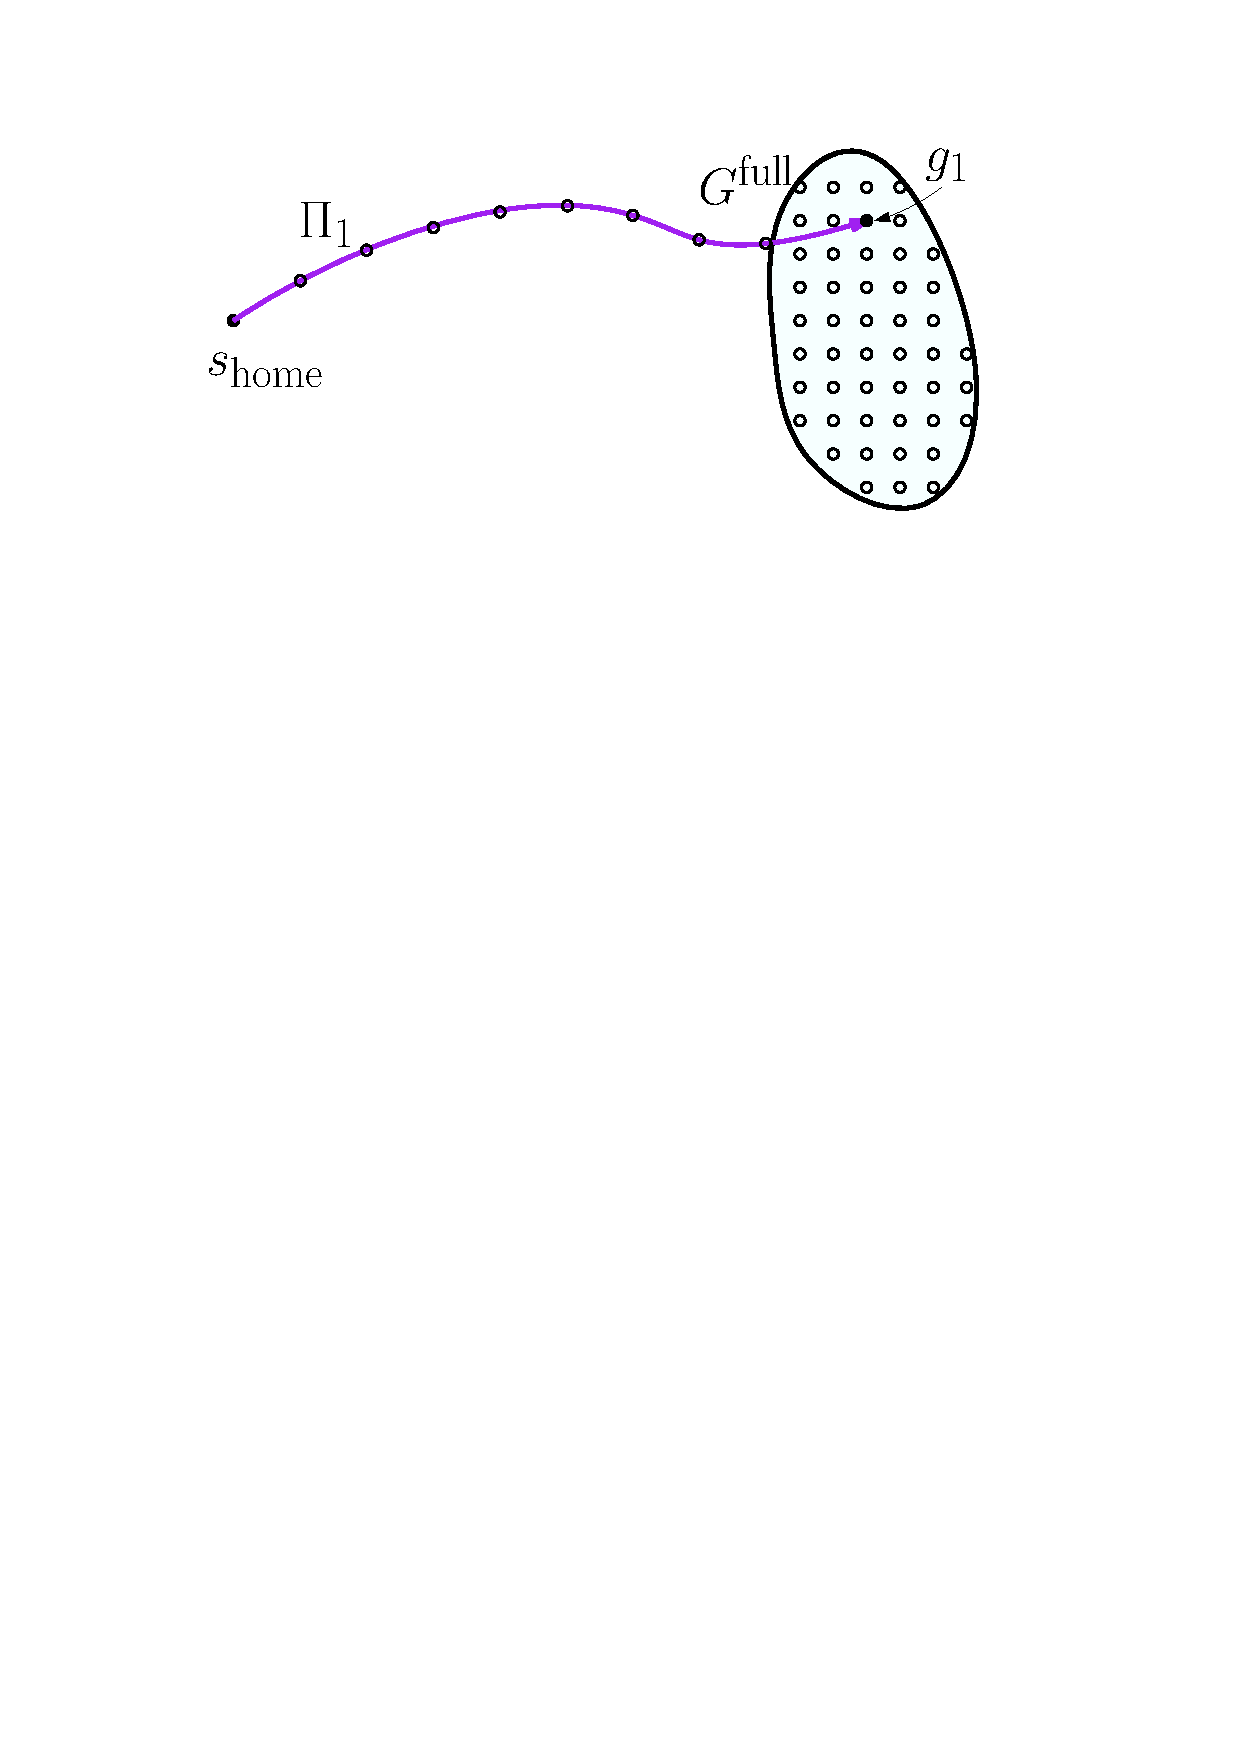
\includegraphics[width=\textwidth]{2_compute_root_paths_1}
        \caption{}
        \label{fig:crp1}
    \end{subfigure}
    \hspace{2mm}
    \begin{subfigure}{0.3\textwidth}
    %   \centering
        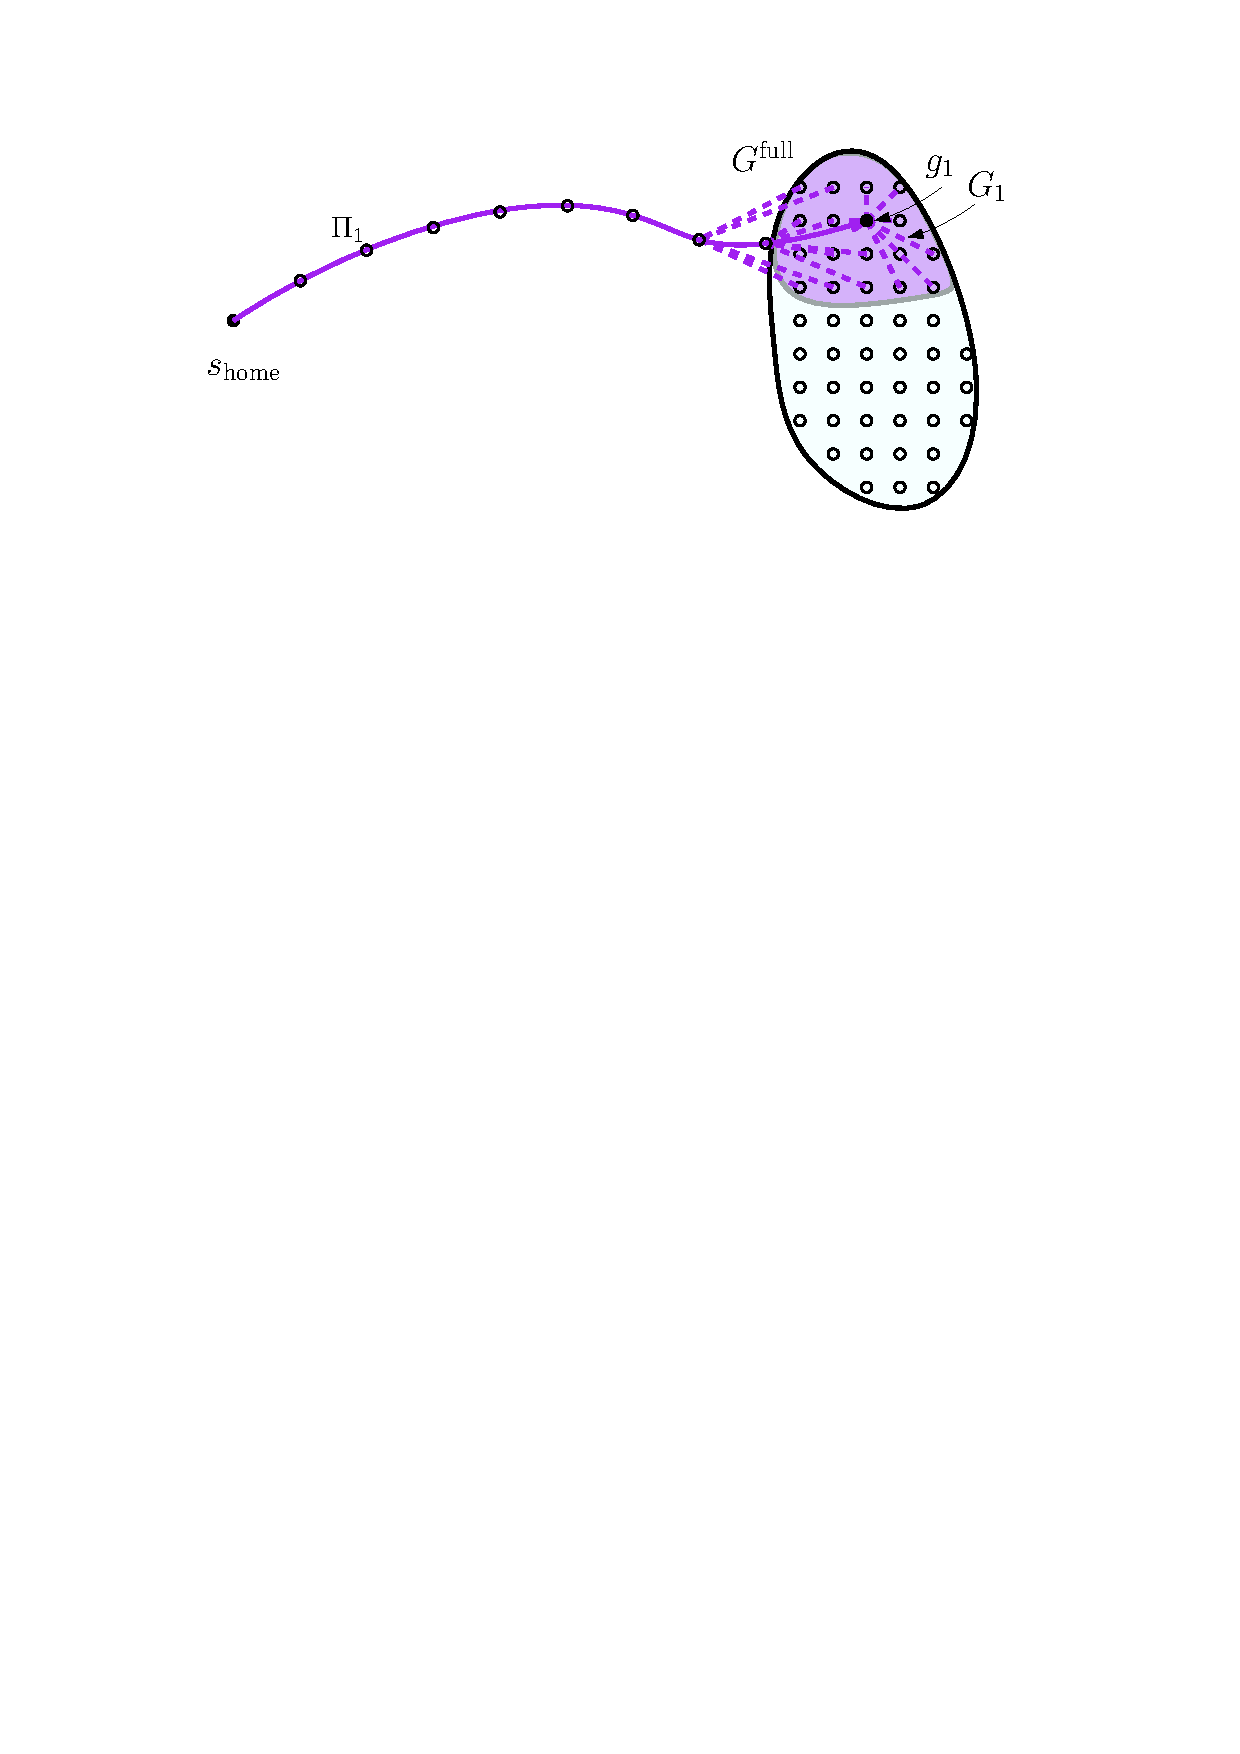
\includegraphics[width=\textwidth]{2_compute_root_paths_2}
        \caption{}
        \label{fig:crp2}
    \end{subfigure}
    \hspace{2mm}
    \begin{subfigure}{0.3\textwidth}
    %   \centering
        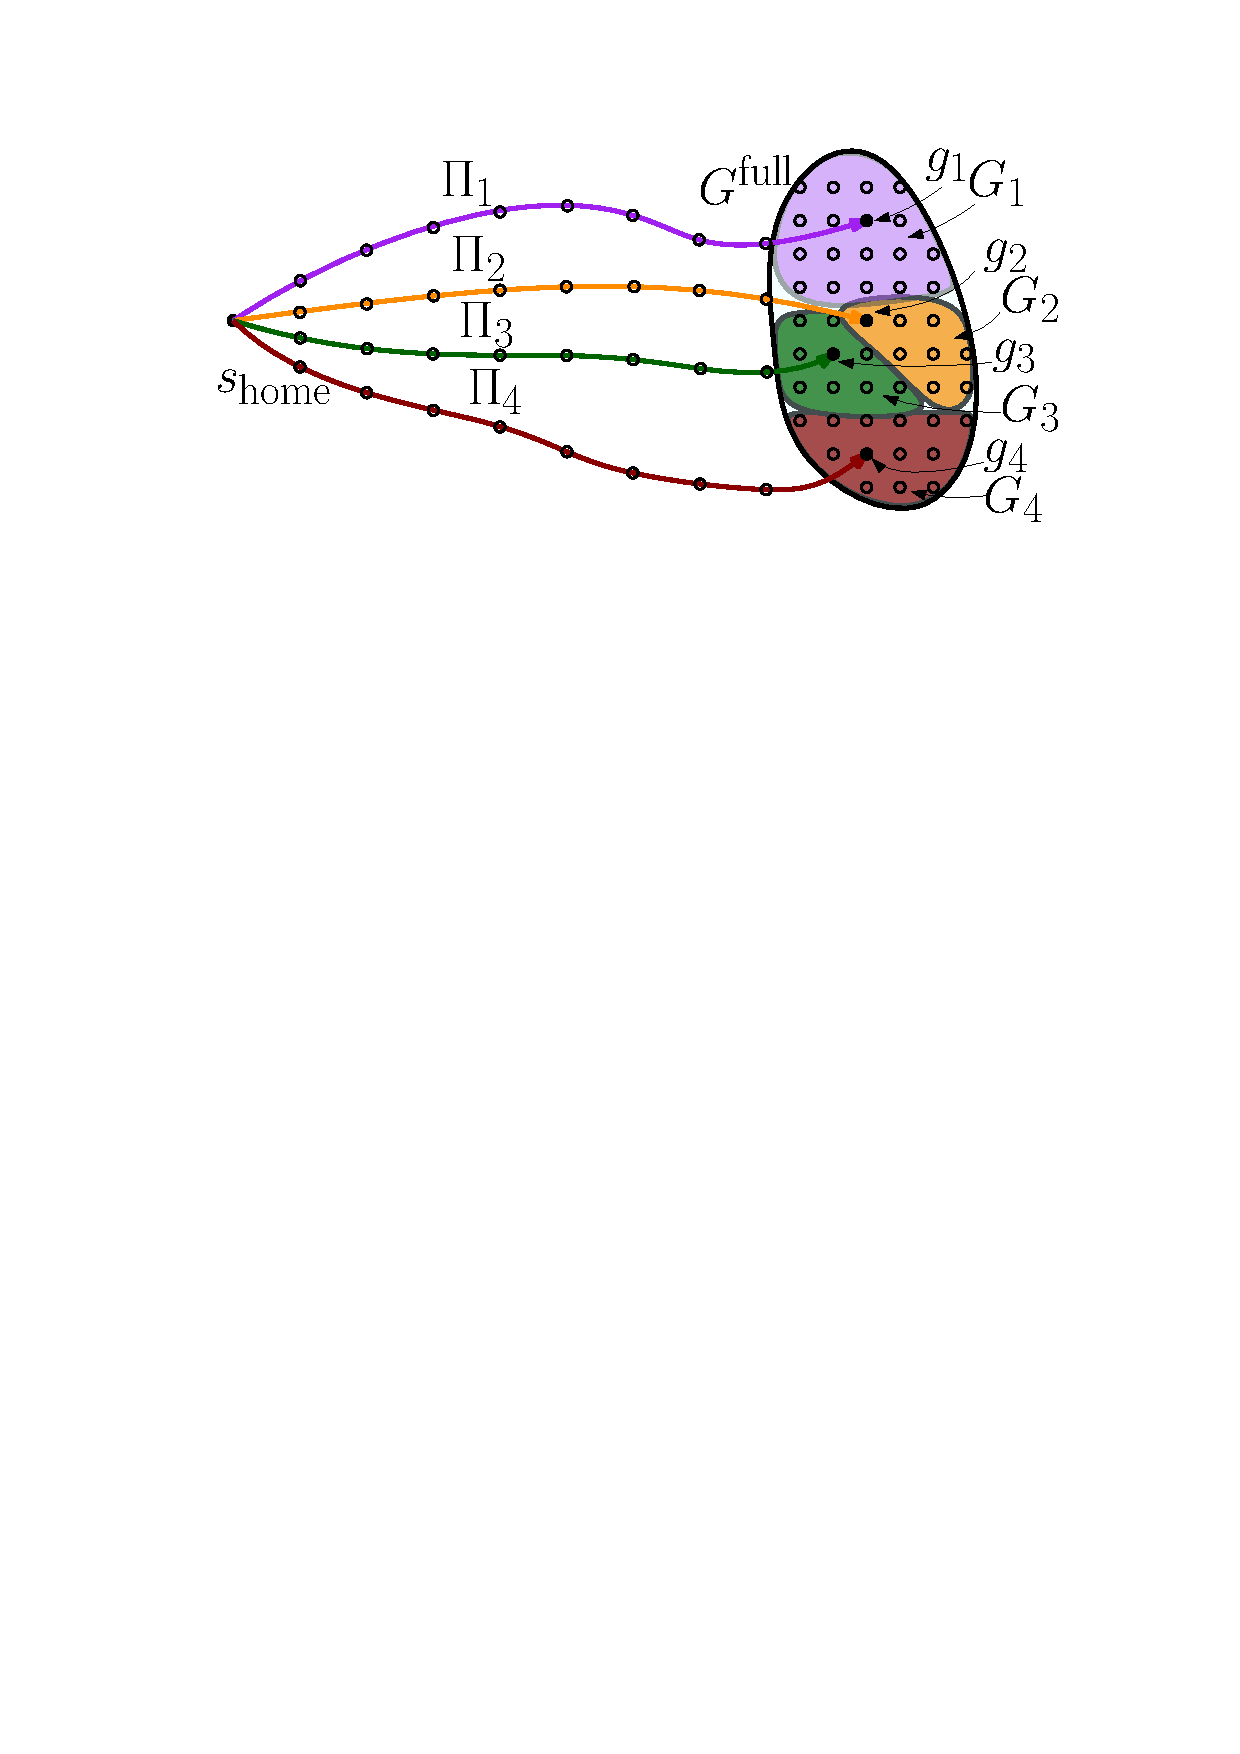
\includegraphics[width=\textwidth]{2_compute_root_paths_3}
        \caption{}
        \label{fig:crp3}
    \end{subfigure}
    \caption{First step of the preprocessing stage.
    (\subref{fig:crp1})~A goal state $g_1$ is sampled and the root path $\Pi_1$ is computed between \Shome and $g_1$.
    %
    (\subref{fig:crp2})~The set $G_1 \subset \Gfull$ of all states that can use $\Pi_1$ as an experience is computed and associated with $\Pi_1$.
    %
    (\subref{fig:crp3})~The goal region covered by four root paths from \Shome after the first step of the preprocessing stage terminates.
    }
    \label{fig:crp}
\end{figure*}

\begin{algorithm}[t]
\caption{\textsc{ComputeRootPaths}($s_{\textrm{start}}, G^{\textrm{UNCOV}}$)}
\label{alg:step1}
\begin{algorithmic}[1]
\State $\Psi \leftarrow \emptyset$   \Comment{A list of pairs ($\Pi, G)$}
\State $G'^{\textrm{UNCOV}} \leftarrow \emptyset$; \hspace{3mm}
       $G'^{\textrm{COV}} \leftarrow \emptyset$; \hspace{3mm}
       $i = 0$
\While{$G^{\textrm{UNCOV}} \neq \emptyset$}
        \Comment{Runs until all uncovered points are considered}
    \State $g_i \leftarrow$\textsc{Sample}($G^{\textrm{UNCOV}}$)
    \State $G^{\textrm{UNCOV}}\leftarrow G^{\textrm{UNCOV}} \setminus \{g_i\}$
    
    \State $\Pi_i \leftarrow$ \textsc{PlanRootPath}($s_{\textrm{start}}, g_i$)
    \If {$\Pi_i = \emptyset$}  \Comment{Path does not exist}
        \State $G'^{\textrm{UNCOV}} \leftarrow G'^{\textrm{UNCOV}} \cup \{g_i\}$
    \Else
        \State $G_i \leftarrow \{ g_i \}$
        \For {\textbf{each} $g_j \in G^{\textrm{UNCOV}}$}
            \State $\pi_j \leftarrow$\textsc{PlanUsingRootPath}($s_{\textrm{start}},g_j,\Pi_i$)
            \If {$\pi_j \neq \emptyset$} \Comment{Planner succeeded}
                \State $G_i \leftarrow G_i \cup \{g_j\}$
                \State $G^{\textrm{UNCOV}} \leftarrow G^{\textrm{UNCOV}} \setminus \{g_j\}$
            \EndIf
        \EndFor
        \State $\Psi \leftarrow \Psi \cup \{ (\Pi_i, G_i)\}$
        \Comment{Insert $(\Pi_i, G_i)$ to $\Psi$}
        \State $i \leftarrow i + 1$
    \EndIf
\EndWhile
\State \textbf{return} $\Psi, G'^{\textrm{UNCOV}}$
\end{algorithmic}
\end{algorithm}

Equipped with a set of root paths and the corresponding goal regions they cover, we now need to allow for efficient replanning. This is done by using the following two observations:
\begin{enumerate}[label={\textbf{O\arabic*}},leftmargin=0.75cm]
    \item \label{obs:1} 
    Assume that the robot is executing a path $\Pi_i$ to $g_i \in G_i$ and that $\Pi_{s, i \rightarrow j}$ is a path starting at state $s \in \Pi_i$ and ending at goal $g_j \in \Gfull \setminus G_i$.
    If the last update given by the perception system happens $\Tbound + \delta_t$ before $s$ is reached,
    then the system can execute path $\Pi_i$ until $s$ and then continue executing $\Pi_{s, i \rightarrow j}$ to reach  $g_j$.

    \item \label{obs:2} 
    Assume that the robot is executing a path $\Pi_i$ to $g_i \in G_i$ and that $\pi_{s,s',i \rightarrow j}$ is a path connecting  $s \in \Pi_i$ to $s' \in \Pi_j$ (with $\Pi_j$ the root path to $g_j \in G_j$).
    If the last update given by the perception system happens $\Tbound + \delta_t$ before~$s$ is reached,
    and the new goal is in $G_j$,
    then the system can execute path $\Pi_i$ until $s$, execute $\pi_{s,s',i \rightarrow j}$ and then continue executing $\Pi_{j}$ from $s'$ until the goal is reached.
    \os{add figure???}
\end{enumerate}

%\subsubsection{Procrastination is a bliss}
%Recall that in the straw man algorithm presented in Sec.~\ref{subsec:strawman}, given a path $\Pi$ connecting \Shome to some goal $g$, we computed a path to every goal state $\Gfull \setminus \{g\}$ from all replanable states.
%
Observation~\ref{obs:1} implies that if we can cover a goal state $g'$  by some state $s$ along $\Pi_g$ (with $g \neq g'$), then we cover $g'$ by all states $\Pi$ that occur before~$s$.
%
Observation~\ref{obs:2} implies that if we can compute a path connecting one root path to some other root path, a process we term as ``latching'' on to the new path, then the new root path can be used to reach all its associated goal states.

We are finally ready to describe the second step of our preprocessing stage.
%
For every root path $\Pi_i$ we look at the last replanning state $s_{\Pi_i, \Trc}$ (namely, the state that is $t=\Trc$ time from \Shome). For every other root path $\Pi_j$, we test if the path connecting $s_{\Pi_i, \Trc}$ to $s_{\Pi_j, \Trc + \delta_t}$ (the state on $\Pi_j$ that is $\Trc+\delta_t$ away from \Shome) is collision free. 
%
If this is the case then all goal states in $G_j$ are covered by all replanning states along $\Pi_i$
%

Let $\Guncov(\Trc)$ be all the states that are still uncovered after the above process. We recursively apply our algorithm to the setting where the start state is $s_{\Pi_i, \Trc}$ and the goal region is $\Guncov(\Trc)$.
If all states are covered after this step, we terminate. 
If not, let $\Guncov(\Trc)'$ be all the states still uncovered.
We consider the state $s_{\Pi_i, \Trc-\delta_t}$ (the state on $\Pi_j$ that is $\Trc-\delta_t$ away from \Shome) and recursively run our algorithm where the start state is $s_{\Pi_i, \Trc-\delta_t}$ and the goal region is $\Guncov(\Trc)'$.
This process is repeated until either all states are covered or we backtracked to \Shome.
For a visualization of this step, see Fig.~\ref{fig:pl}.
For pseudocode see Alg.~\ref{alg:all} and~\ref{alg:step1}.

Thus, the outcome of the preprocessing stage is map $\calM: S \times \Gfull \rightarrow \{ \Pi_1, \P_2, \ldots \}$ mapping which root path can be as an expirience to reach a goal $g$ from a state $s$.
%
In addition \os{WHAT ABOUT SNAPPING MOTIONS???}

\subsubsection{Query}
In the query stage, given an initial estimation $g_{\rm init}$ of the goal pose from $\calP$, our algorithm queries $\calM$ to obtain the root path $\Pi$ from $\Shome$ to $g_{\rm init}$.
It then plans a path using $\Pi$ as an experience and starts executing this path.
%
Now, assume that the~$\calR$ is executing path $\Pi_{\rm curr}$ and a new estimation $g_{\rm new}$ of the goal pose is provided by $\calP$.
%
We consider the state $s_{\Pi_{\rm curr}, \Trc}$ along the path $\Pi_{\rm curr}$ at time $\Trc$ and test if
(i)~there is a root path that can be used as an experience to reach $g_{\rm new}$ starting at $s_{\Pi_{\rm curr}, \Trc}$
of if 
(ii)~there is another root path associated with $g_{\rm new}$ that we can latch on to \os{this needs some elaboration}.
If the former holds, we run our experience-based planner to obtain a path $\Pi(s_{\Pi_{\rm curr}}, \Trc, g_{\rm new})$ starting at $s_{\Pi_{\rm curr}}$ and ending at $g_{\rm new}$. We then execute $\Pi_{\rm curr}$ until $s_{\Pi_{\rm curr}, \Trc}$ and then continue by executing $\Pi(s_{\Pi_{\rm curr}}, \Trc, g_{\rm new})$.
%
If the latter holds, we run our experience-based planner to obtain a path $\Pi(s', \Trc + \delta_t), g_{\rm new})$ starting at $s'$, the state on the path we latched on to and ending at $g_{\rm new}$. We then execute $\Pi_{\rm curr}$ until $s_{\Pi_{\rm curr}, \Trc}$ and then continue by executing the motion that latches on to $s'$ and finaly executing  $\Pi(s', \Trc + \delta_t, g_{\rm new})$.
%
If neither hold, we condider the state $s_{\Pi_{\rm curr}, \Trc-\delta_t}$ and repeat this process.
%
For pseudocode describing our approach see~\ref{alg:query}.

\subsection{Bounded-time guarantees}
\os{Fahad - can you sketch something here?}
\begin{algorithm}
\caption{\textsc{PreprocessMain(\Shome, \Gfull)}}\label{alg:all}
\begin{algorithmic}[1]
\State \textsc{Preprocess}($\Shome, \Gfull$)
\end{algorithmic}
\end{algorithm}


\ignore{
Before describing how this is done, consider two root paths $\Pi_i$ and $\Pi_j$ with associated goal regions $G_i$ and~$G_j$, respectively.
Now, let $s_i$ and $s_j$ be states on $\Pi_i$ and $\Pi_j$, respectively, such that the timestamp associated with $s_j$ is $\delta_t$ time after the one associated with $s_i$. Furthermore, assume that the path between $s_i$ and $s_j$ is collision free. 
%
Now, assume that the robot is executing path $\Pi_i$ (targeting a goal state in $G_i$) and the perception system updates the goal state to be reached as $g_j \in G_j$. 
If the robot did not yet reach $s_i$ then it can reach $g_j$ by
(i)~continuing to follow $\Pi_i$ until $s_i$ is reached, 
(ii)~move to $s_j$ on $\Pi_j$ and 
(iii)~use $\Pi_j$ to reach $g_j$.
%
We term the process we just described of moving from one root path to another as ``latching'' on to a new root path.

Let $s_{\Pi_i, t}$ be the state that is $t$ time from \Shome on path $\Pi_i$.
If a collision-free path existed from $s_{\Pi_i, \Trc}$ to $s_{\Pi_j, \Trc+\delta_t}$ for every $i,j$ then we could latch on from any root path to any other root path. Moreover, following Assumption~\ref{assum:4}, $\Trc$ is the last time that the perception could update the goal location so no other replanning would be required.
%
Unfortunately, this may not be the case.
%
Thus, for every root path $\Pi_i$, we consider $s_{\Pi_i, \Trc}$ and check if we can latch on to all other root paths. 
If this can't be done, then we can tr

considering the last replanning state $s_{\Pi_i, \Trc}$ (namely, the state that is $t=\Trc$ time from \Shome). For every other root path $\Pi_j$, we test if the path connecting $s_{\Pi_i, \Trc}$ to $s_{\Pi_j, \Trc + \delta_t}$ (the state on $\Pi_j$ that is $\Trc+\delta_t$ away from \Shome) is collision free. 

In the straw man algorithm this was obtained by recursively computing a path for the replanning states along all the previously-computed paths.
%
Here, we attempt to re-use the previously-computed paths as much as possible by ``latching'' onto them.




More formally, for each root path~$\Pi_i$, we start by considering the last replanning state $s_{\Pi_i, \Trc}$ (namely, the state that is $t=\Trc$ time from \Shome). For every other root path $\Pi_j$, we test if the path connecting $s_{\Pi_i, \Trc}$ to $s_{\Pi_j, \Trc + \delta_t}$ (the state on $\Pi_j$ that is $\Trc+\delta_t$ away from \Shome) is collision free. 
If this is the case we know that any goal state in $G_j$ can be
}

%%%%%%%%%%%%%%%%%%%%%%%%%%%%%%%%%%%%%%%%%%%%%%%%%%%%
\begin{algorithm}
\caption{\textsc{Preprocess}($\Sstart,\Guncov,\Gcov $)}\label{alg:2}
\begin{algorithmic}[1]
\State $\Psi_{\textrm{work}}, G'^{\textrm{uncov}}_{\textrm{work}} \leftarrow$ \textsc{ComputeRootPaths}($\Sstart,\Guncov$)

\If {$\Sstart = \Shome$}
    \State $\Psi_{\textrm{home}} = \Psi_{\textrm{work}}$
\EndIf

\State $G'^{\textrm{cov}} \leftarrow 
    \Gcov \cup (\Guncov \setminus G'^{\textrm{uncov}}_{\textrm{work}})$
\If{$t(s_{\textrm{start}}) \geq \Trc$}
    \State \textbf{return} $G'^{\textrm{uncov}}_{\textrm{work}}, G'^{\textrm{cov}}$
\EndIf
\For {\textbf{each} $(\Pi_i, G_i) \in \Psi_{\textrm{work}}$}
    \State $G_i^{\textrm{cov}} \leftarrow G_i$;
            \hspace{2mm}
           $G_i^{\textrm{uncov}} \leftarrow G'^{\textrm{cov}} \setminus G_i$;
            \hspace{2mm}
           $t = \Trc$
%    \State $t = \Trc$
%    \State $G_i^{\textrm{UNCOV}} \leftarrow G'^{\textrm{COV}} \setminus G_i$
%    \State $G_i^{\textrm{COV}} \leftarrow G_i$

    \While{$t \geq t(\Sstart)$}
        \State $s \leftarrow$ \textsc{GetState($\Pi_i, t$)}
        \For {\textbf{each} $(\Pi_j, G_j) \in \Psi_{\textrm{home}}$}
            \If{\textsc{CheckSnap}($s,\Pi_j$)}
                \State $G_i^{\textrm{uncov}} \leftarrow G_i^{\textrm{uncov}} \setminus G_j$
                \State $G_i^{\textrm{cov}} \leftarrow G_i^{\textrm{cov}} \cup G_j$
            \EndIf
        \EndFor
        % }
        %%%%%%%%% LATCHING END
        \If{$G_i^{\textrm{uncov}} = \emptyset$}
            \State \textbf{break}
        \EndIf
        \State $G_i^{\textrm{uncov}},G_i^{\textrm{cov}} \leftarrow$ \textsc{Preprocess}($s,G_i^{\textrm{uncov}},G_i^{\textrm{cov}}$)
        \If{$G_i^{\textrm{uncov}} = \emptyset$}
            \State \textbf{break}
        \EndIf
        \State $t \leftarrow t - \delta_t$
    \EndWhile
    % \State $(\Pi_i,\Pi_j).s = s$ \Comment{replan state}
\EndFor
\State \textbf{return} $G'^{\textrm{uncov}}_{\textrm{work}}, G'^{\textrm{cov}}$

\end{algorithmic}
\end{algorithm}

%%%%%%%%%%%%%%%%%%%%%%%%%%%%%%%%%%%%%%%%%%%%%%%%%%%%





\begin{figure*}[t]
    \centering
    \begin{subfigure}{.225\textwidth}
    %   \centering
        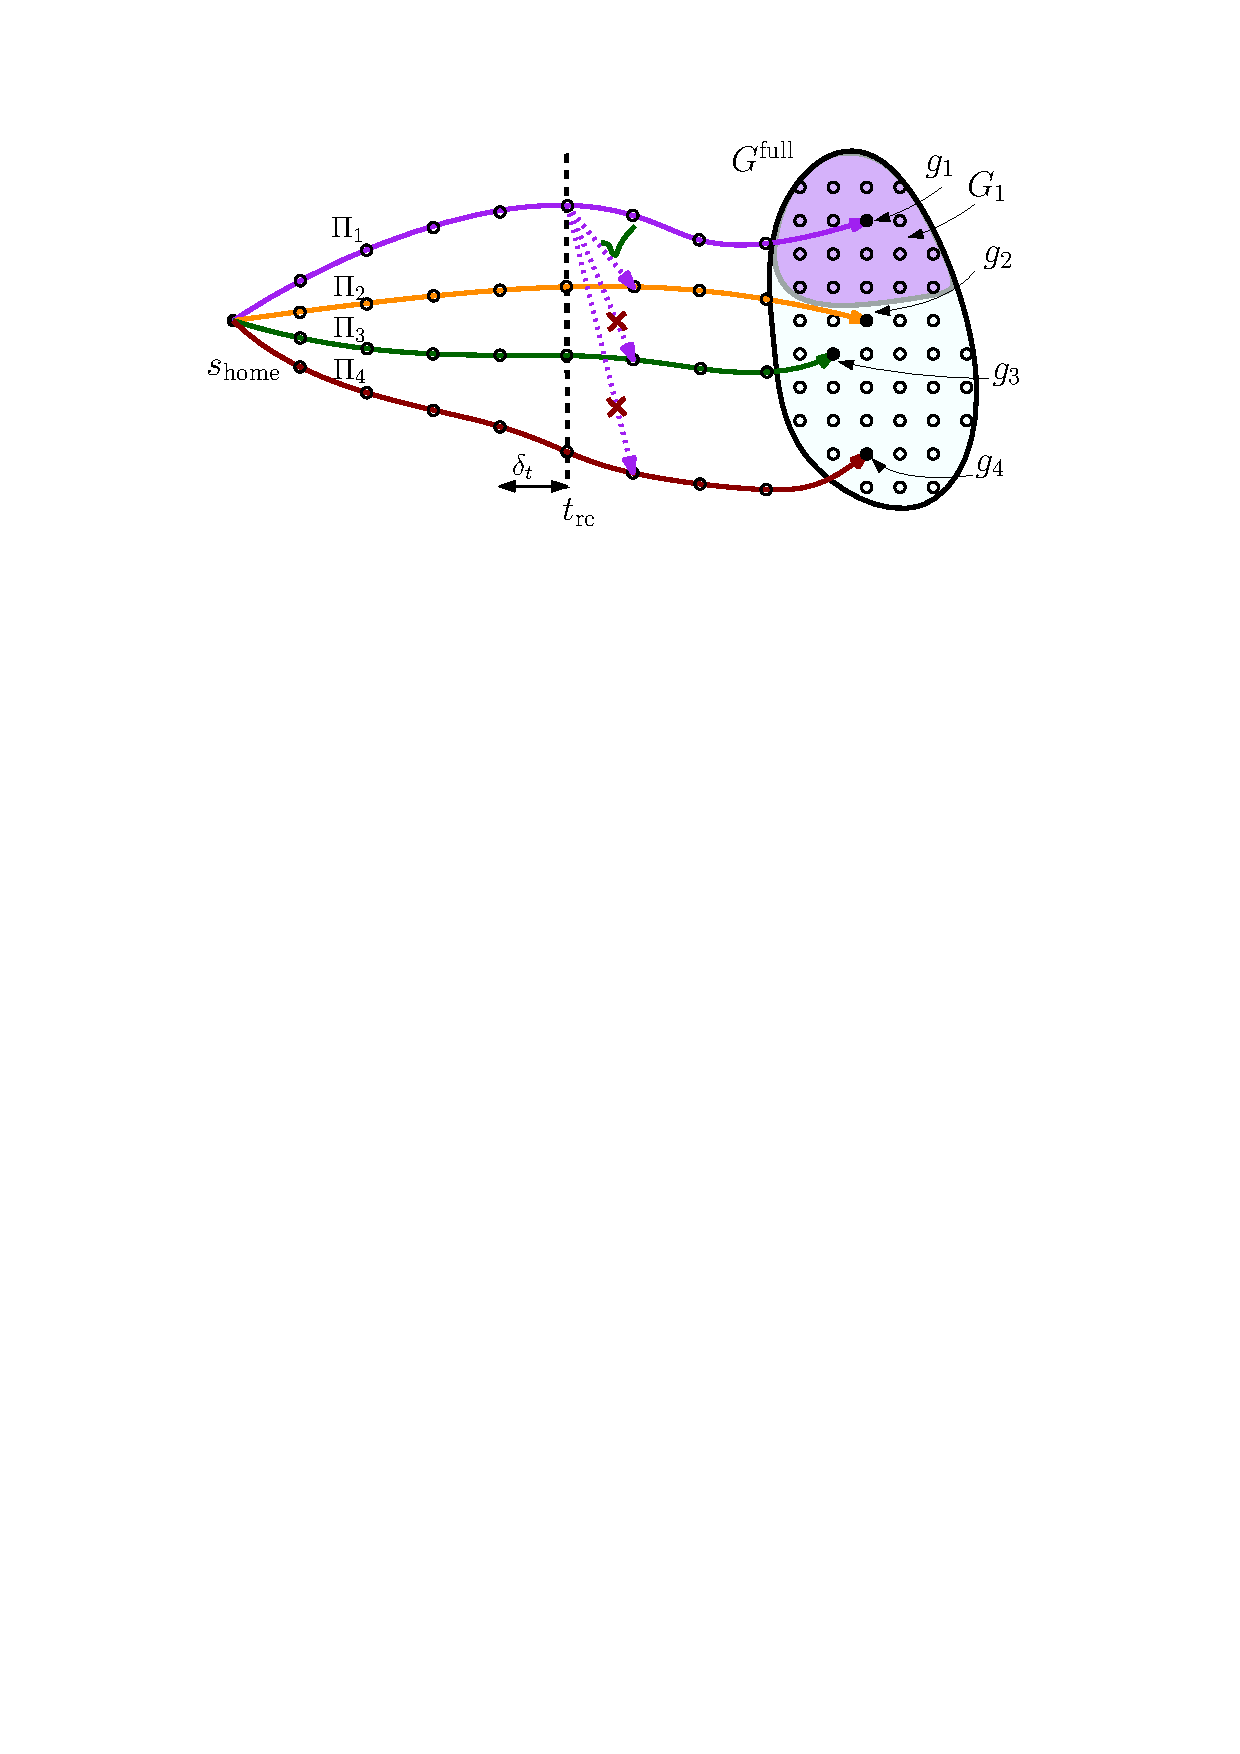
\includegraphics[width=\textwidth]{3_preprocess_loop_1}
        \caption{}
        \label{fig:pl1}
    \end{subfigure}
    \hspace{1mm}
    \begin{subfigure}{0.225\textwidth}
    %   \centering
        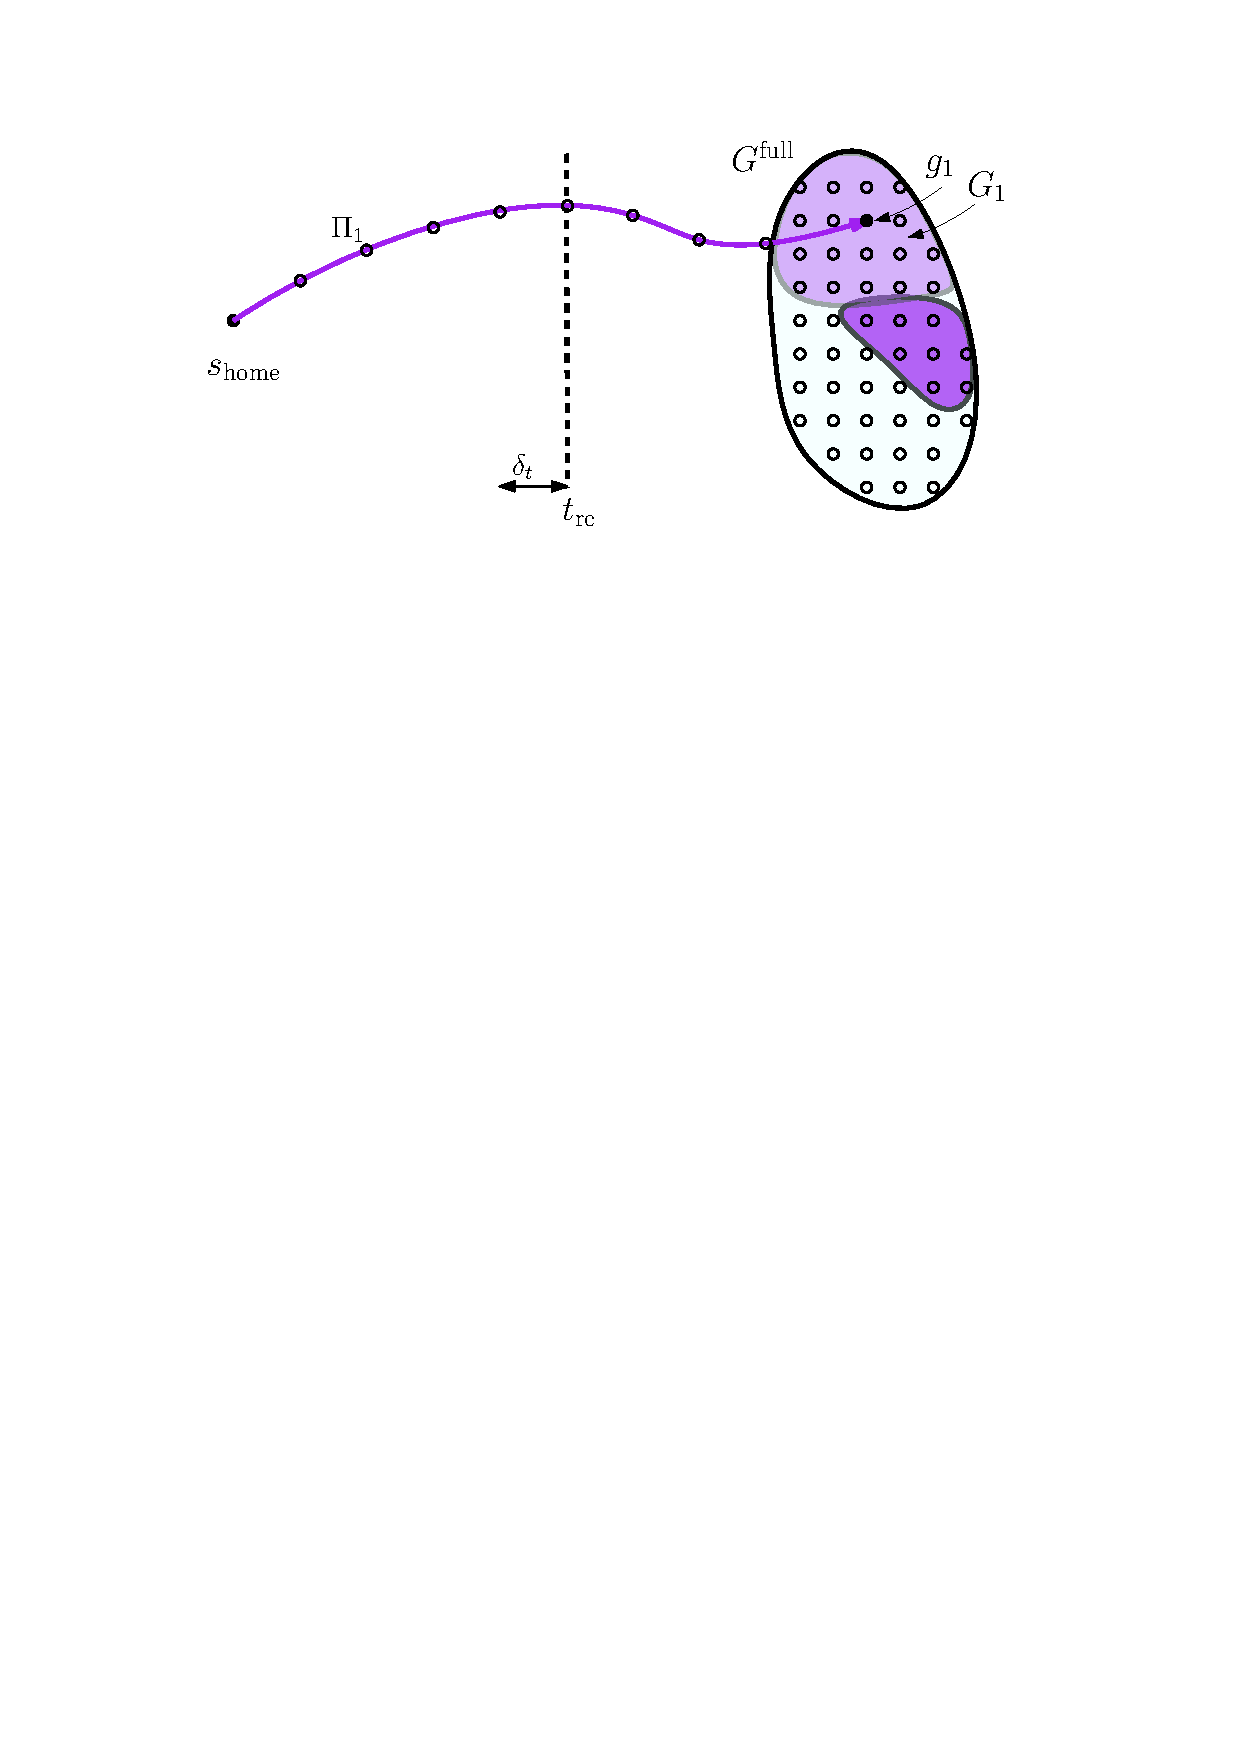
\includegraphics[width=\textwidth]{3_preprocess_loop_2}
        \caption{}
        \label{fig:pl2}
    \end{subfigure} 
    \hspace{1mm}
    \begin{subfigure}{0.225\textwidth}
    %   \centering
        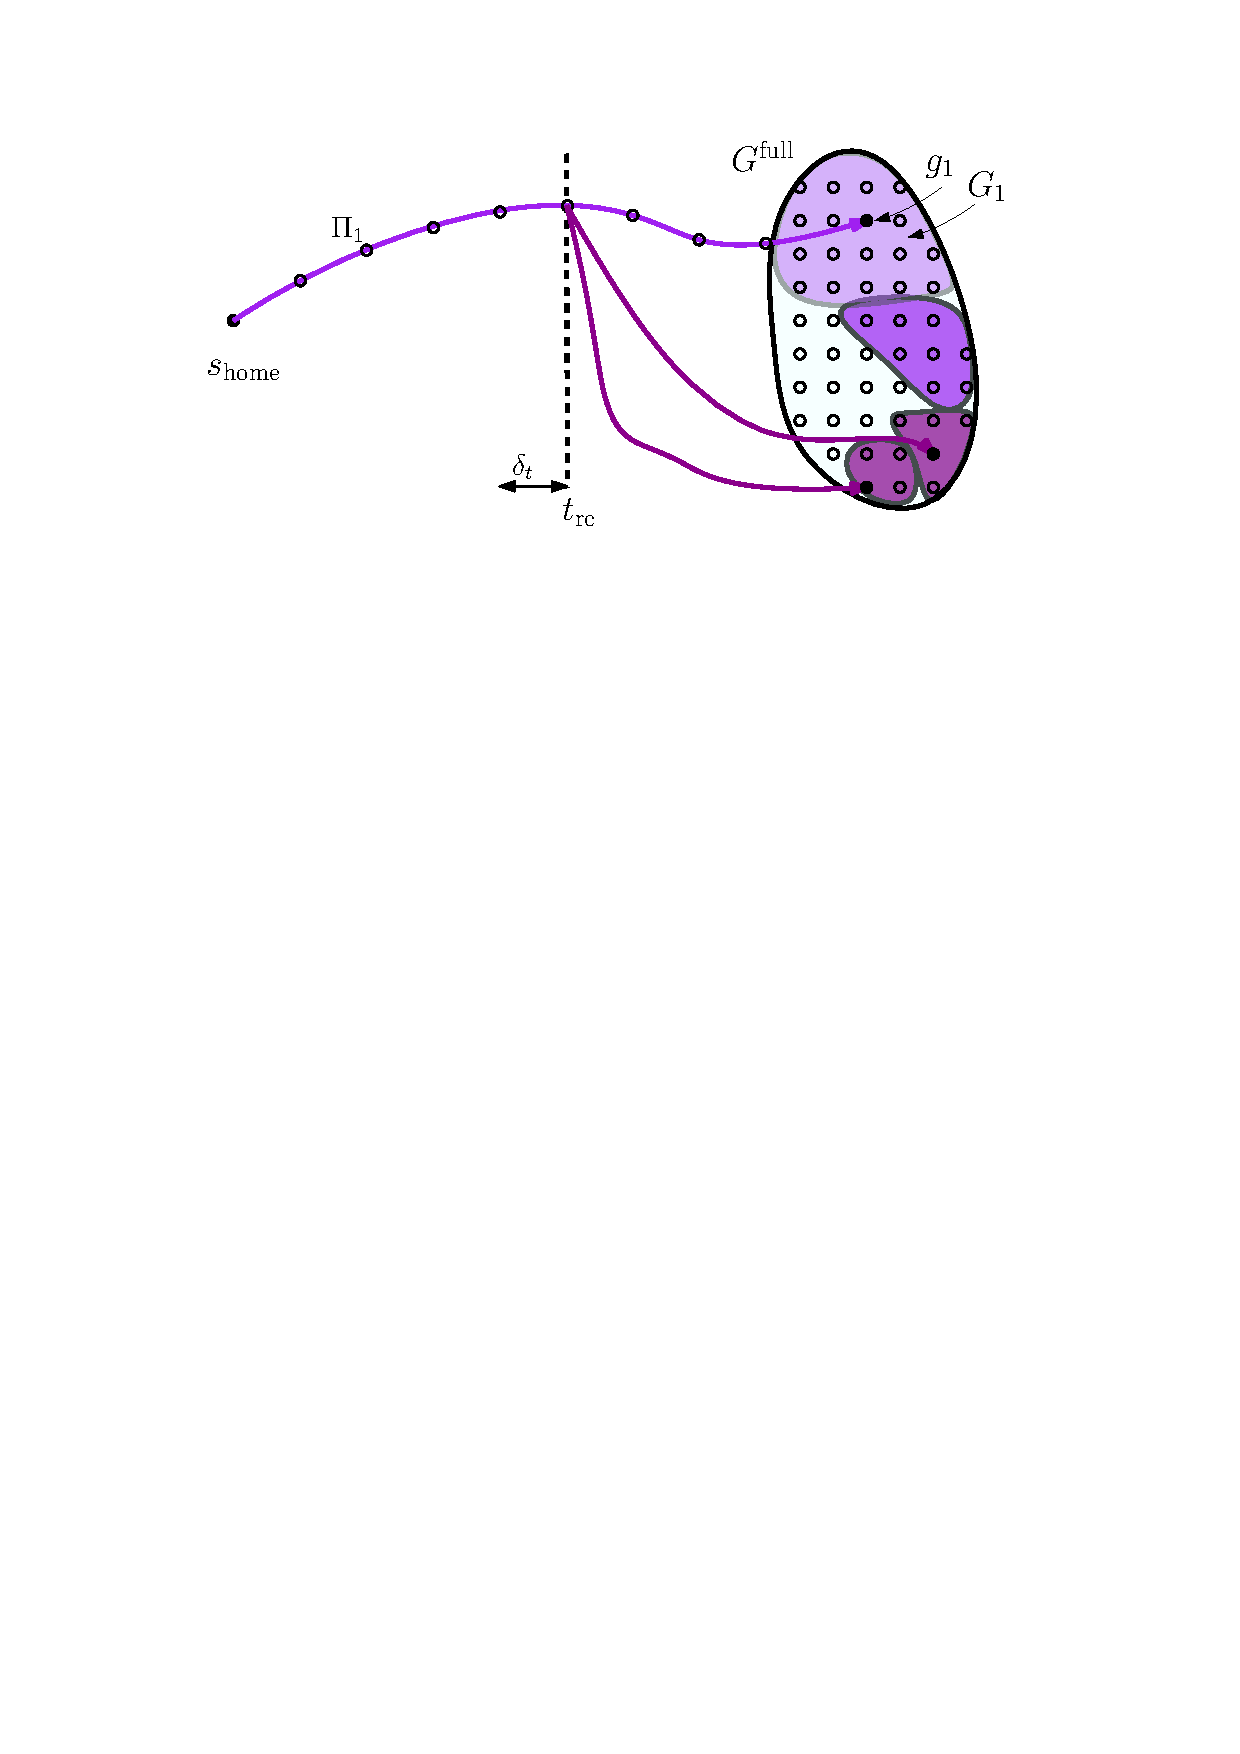
\includegraphics[width=\textwidth]{3_preprocess_loop_3}
        \caption{}
        \label{fig:pl3}
    \end{subfigure}
    %
    \hspace{1mm}
    \begin{subfigure}{.225\textwidth}
    %   \centering
        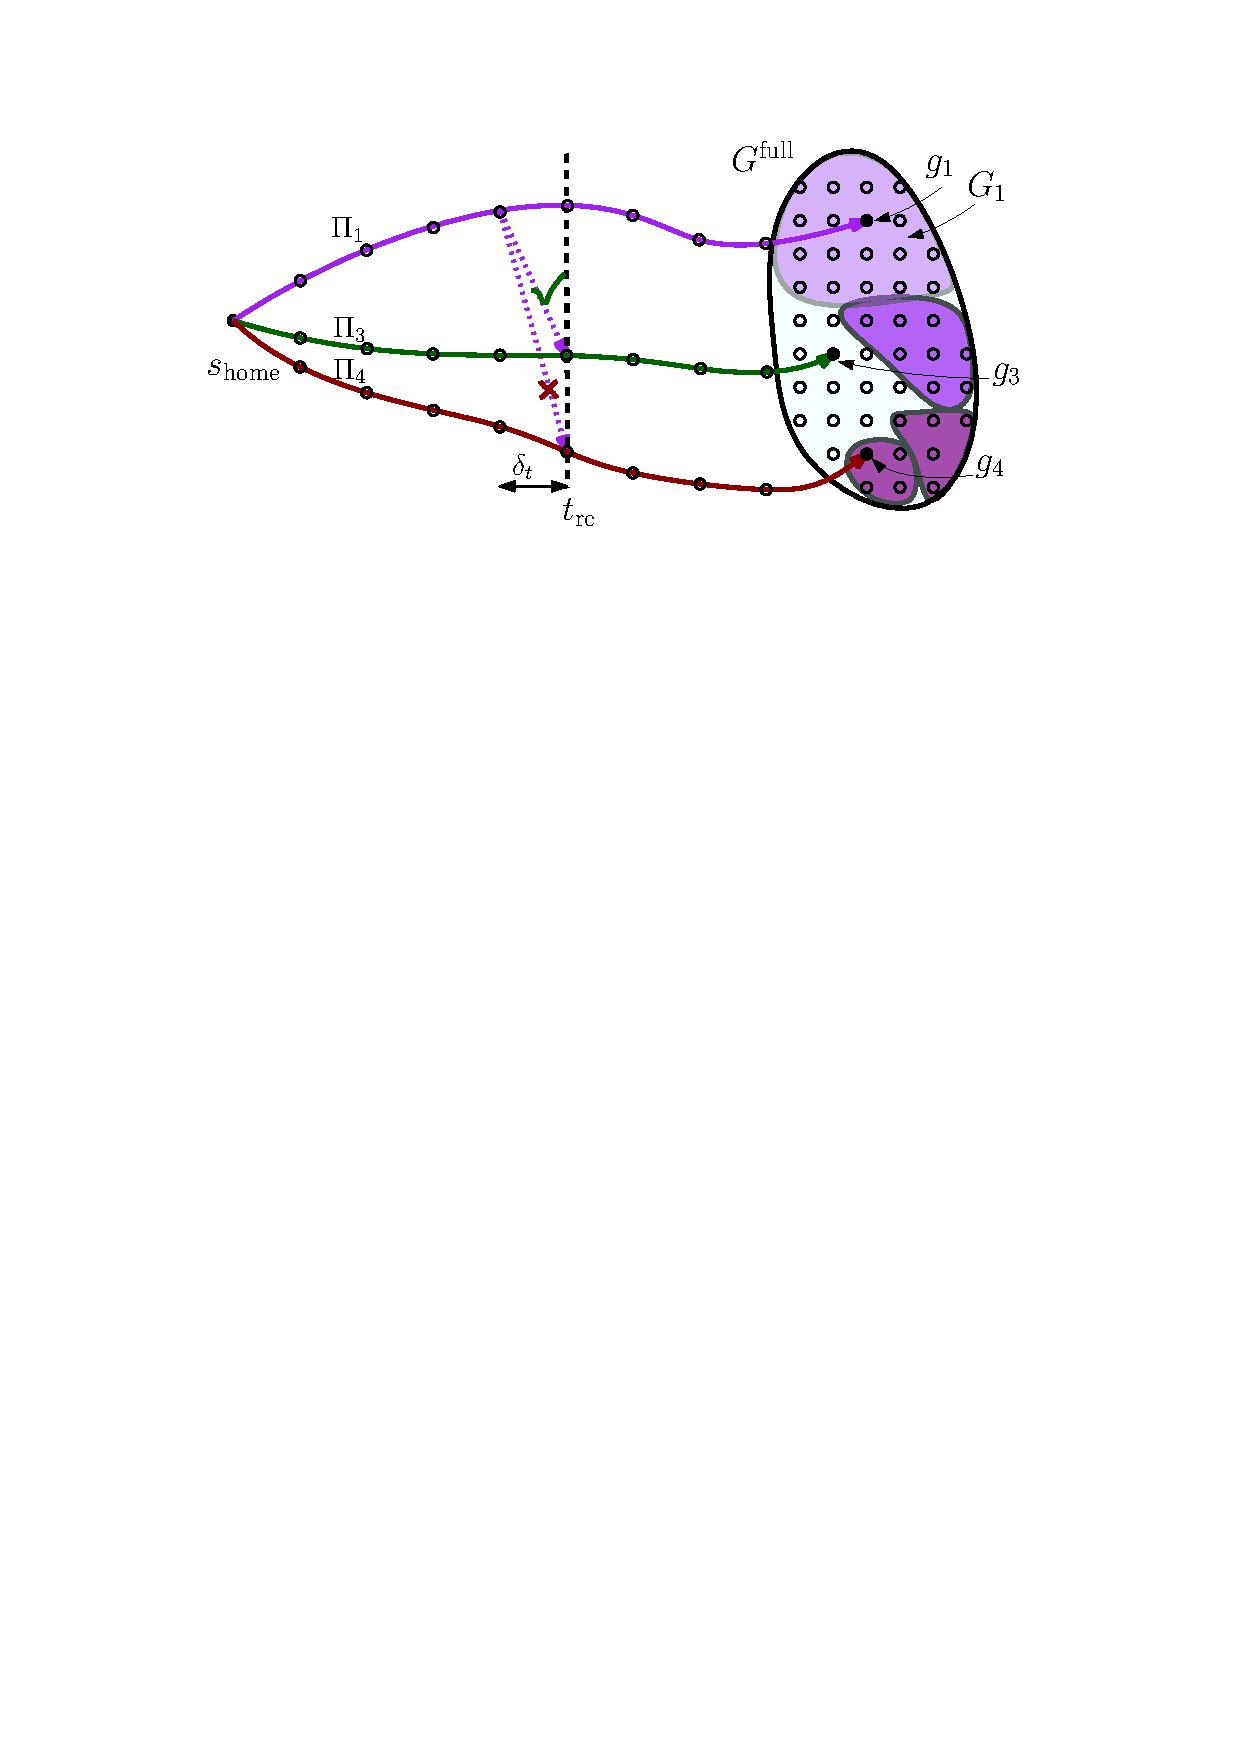
\includegraphics[width=\textwidth]{3_preprocess_loop_4}
        \caption{}
        \label{fig:pl4}
    \end{subfigure}
    %\hspace{2mm}
    \begin{subfigure}{0.225\textwidth}
    %   \centering
        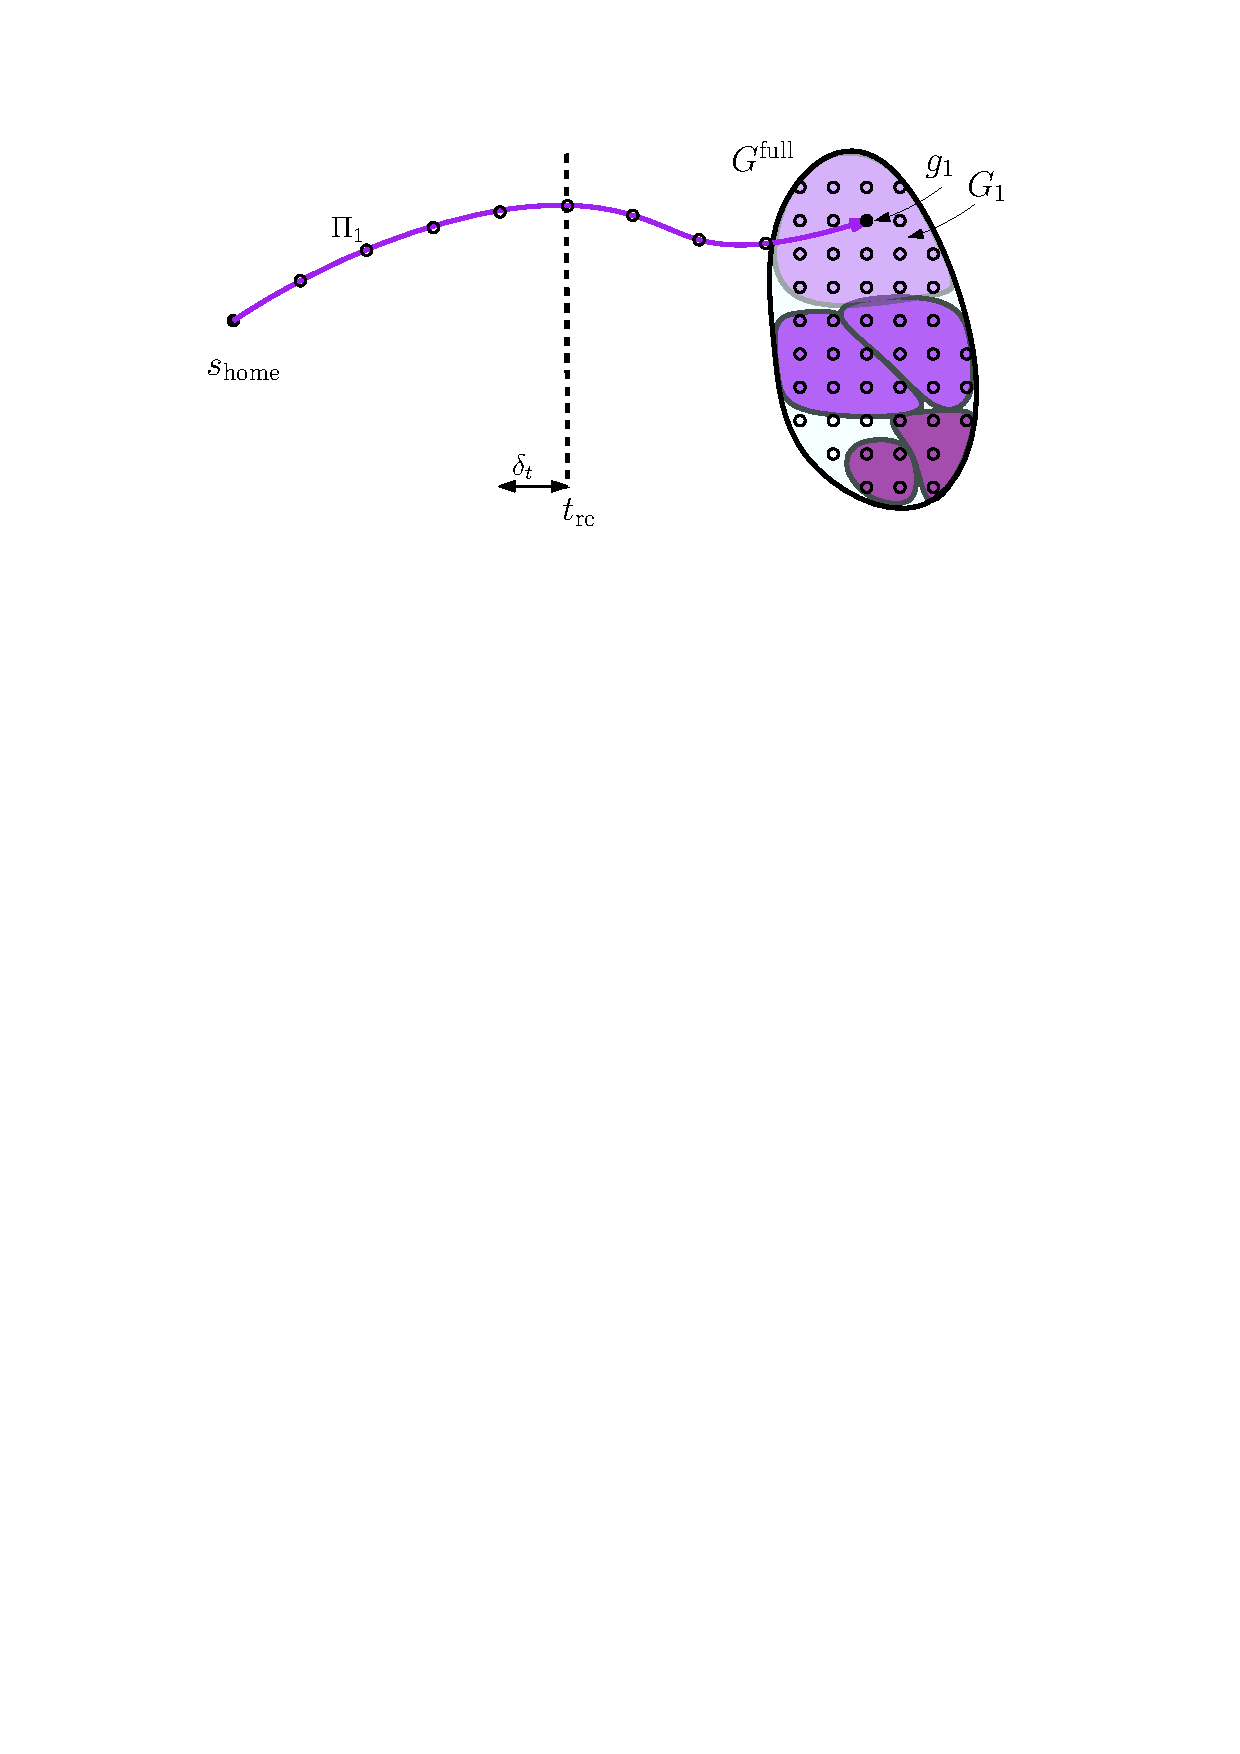
\includegraphics[width=\textwidth]{3_preprocess_loop_5}
        \caption{}
        \label{fig:pl5}
    \end{subfigure}
    \hspace{1mm}
    \begin{subfigure}{0.225\textwidth}
    %   \centering
        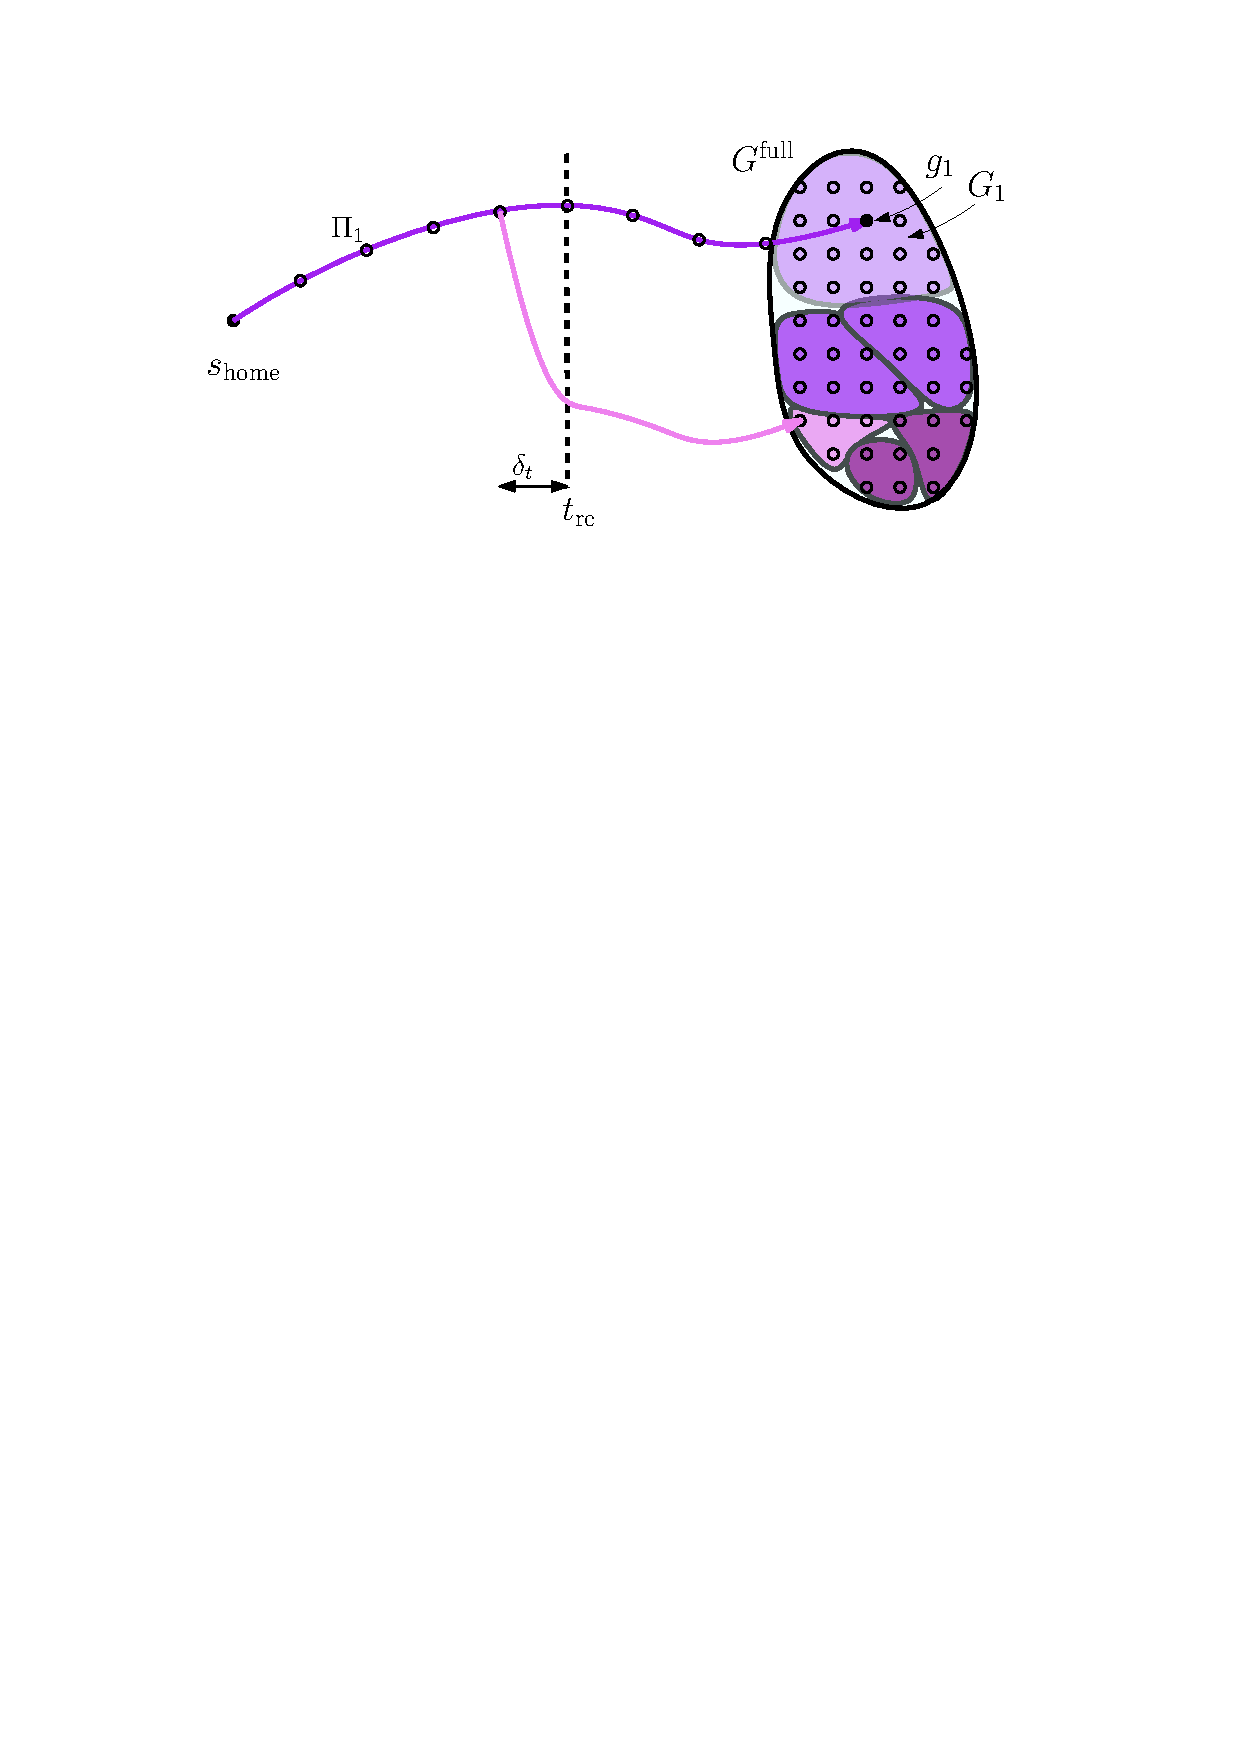
\includegraphics[width=\textwidth]{3_preprocess_loop_6}
        \caption{}
        \label{fig:pl6}
    \end{subfigure}
    \hspace{1mm}
    \begin{subfigure}{0.225\textwidth}
    %   \centering
        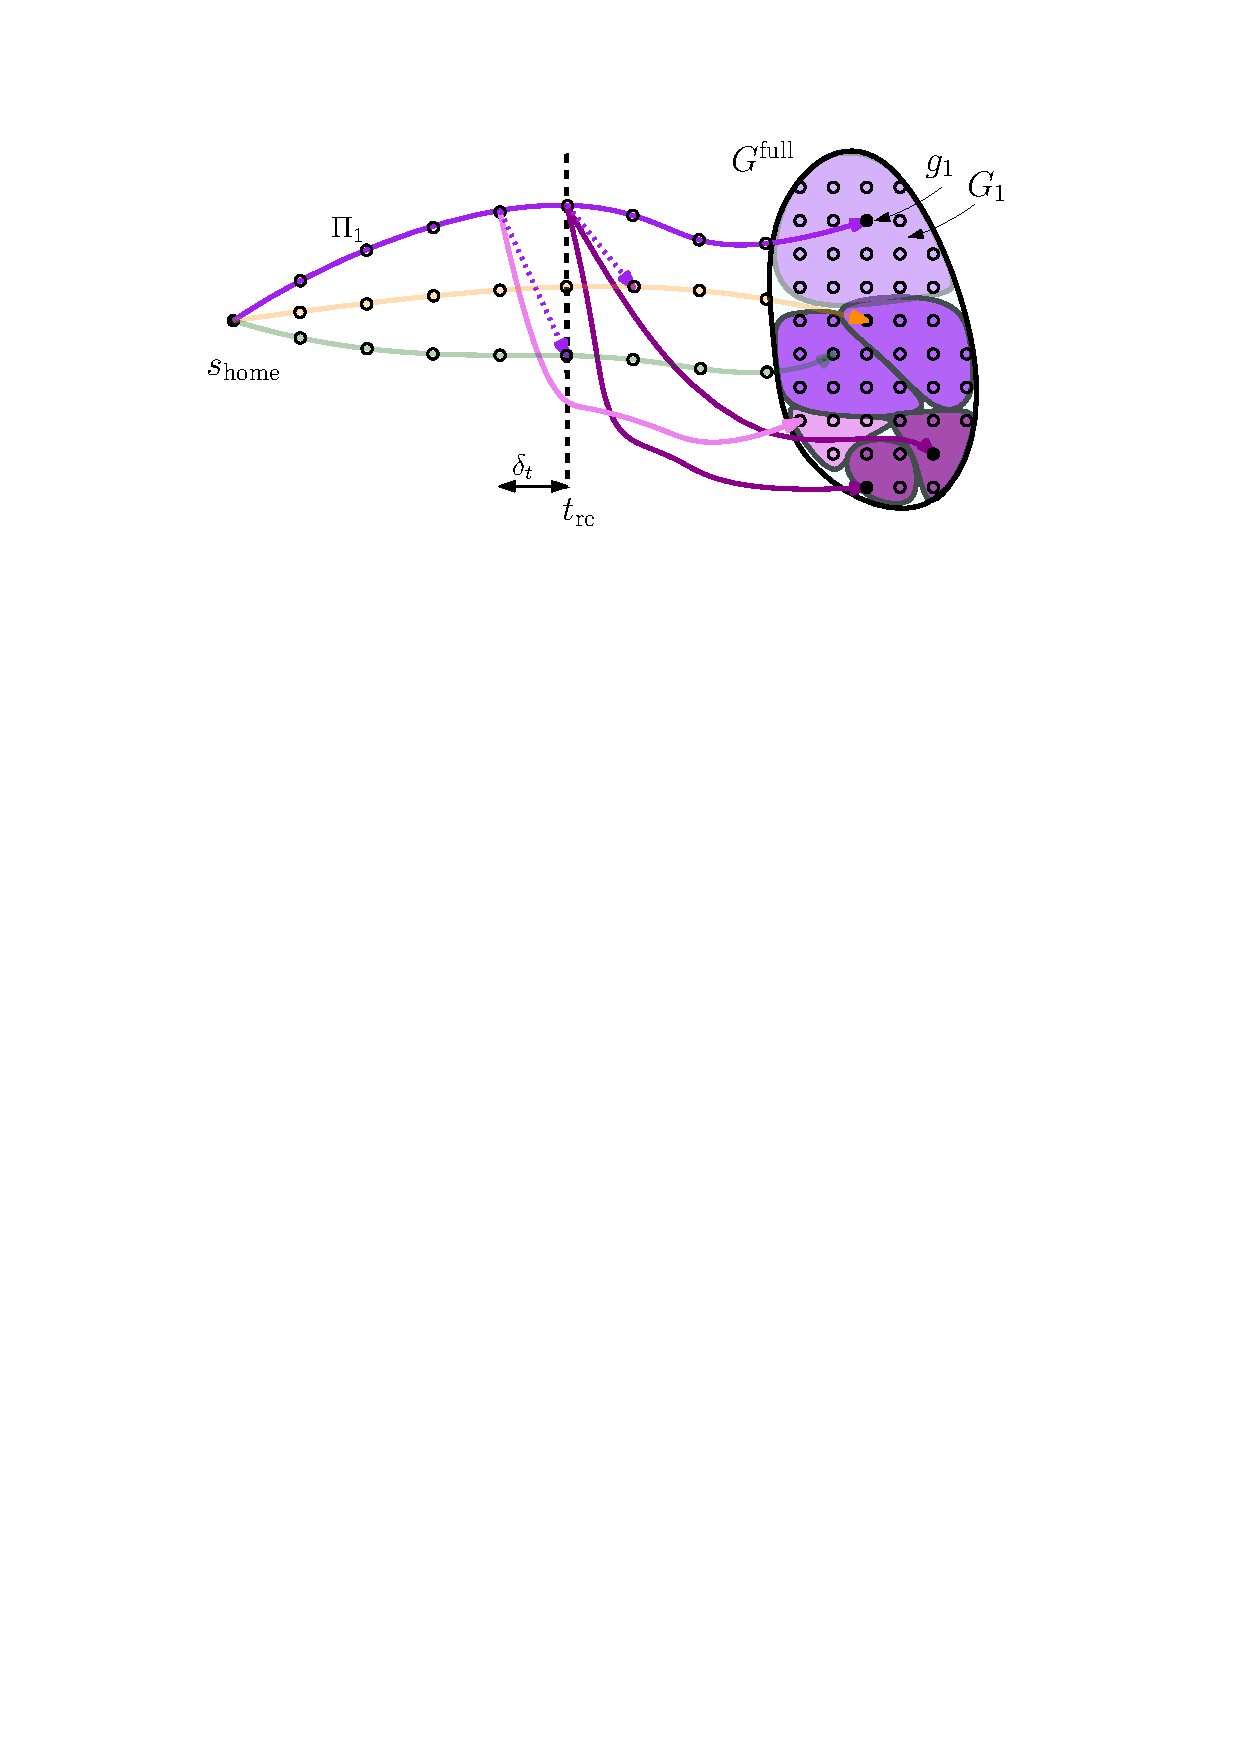
\includegraphics[width=\textwidth]{3_preprocess_loop_7}
        \caption{}
        \label{fig:pl7}
    \end{subfigure}
    \caption{Preprocess loop
    (\subref{fig:pl1})~text.
    %
    (\subref{fig:pl2})~text.
    %
    (\subref{fig:pl3})~text.
    \os{update text}
    }
    \label{fig:pl}
\end{figure*}

\section{Evaluation}
\label{sec:eval}

\section{Conclusion \& future work}

\section*{Acknowledgments}

\vfill
\pagebreak
\section{Algorithm}

\subsection{Problem Definition and Assumptions}
We define a goal region $G^{\textrm{full}}$ as a discretized set of initial object poses on the conveyor belt that the robot can perceive when the object comes in its field of view. Given a home configuration for the robot $s_{\textrm{home}}$, we want to be able to plan for any goal pose $g_{\textrm{init}}$ in bounded time $t_{\textrm{bound}}$. The perception system is setup such that it sends updated pose estimates on the fly during execution as it gets better estimates over time. Given any current state of the robot during execution $s_{\textrm{start}}$, the planner should be able to replan from $s_{\textrm{start}}$ to any subsequent goal $g_{\textrm{next}}$.

We make the following assumptions about the system.
\begin{itemize}
\item $G^{\textrm{full}}$ would accommodate for an error $\epsilon$ in the initial pose estimate $g_{\textrm{init}}$ of the perception system. Each subsequent estimate $g_{\textrm{next}}$ will be within the $\epsilon$ window around $g_{\textrm{init}}$ (in retrospect because the conveyor is moving).
\item We assume that all $\forall g \in G^{\textrm{full}}$, there exists a path from $s_{\textrm{home}}$ to $g$ and we can find it in finite preprocessing time (not sure about this one)
\item We assume that the reachable set of goals for a state on a path is a subset of the reachable set of every other state on that path that exists before it.
\item There exists a replan cutoff time $\Trc$ from when the robot starts moving, after which the planner does not accept more replanning requests.
\item We assume that before $\Trc$, the environment is static. In other words the moving target object cannot collide with the robot during that time.
\end{itemize}

\subsection{Properties}
\begin{itemize}
\item The planning time for each planning/replanning request is bounded ($t_{\textrm{bound}}$)
\item We discretize the trajectories with the resolution $\delta t$. The reaction time of the robot to a replanning request is bounded by $t_{\textrm{bound}} + \delta t$
\end{itemize}

\subsection{Offline Motion Planner}
In this section we will describe the motion planner that is used in the \textsc{PlanPath()} and \textsc{PlanPathUsingRootPath()} functions in Algs.~\ref{alg:3} and~\ref{alg:4}. We use a heuristic search based planning approach with motion primitives (cite papers here). There are a few advantages of this approach for our particular problem.
\begin{itemize}
    \item It can elegantly handle under-defined goals. We define a goal as a 6DOF grasp pose for the goal object. The goal is underdefined as there is a redundant degree of freedom of the robot and also because the grasping time is not specified.
    \item We make use of a set of predefined motion primitives and dynamically generated motion primitives which can be computed such that the kinodynamic constraints of the robot are respected. These primitives are used to generate an implicit graph which is searched by a heuristic search-based planner to compute a plan
    \item We can design informative heuristic functions to speed up the search
    \item We use an existing search-based algorithm e-graphs (cite here) that reuses past experiences and significantly reduces planning times for repetitive tasks
\end{itemize}


\subsubsection{State Space and Graph Construction}

Let $G = (S,E)$ denote an implicit directed graph that we construct, where $S$ denotes the states on $E$ denotes the directed edges that define the transition between this states. A state $s$ in $S$ is uniquely defined by the tuple ($\mathcal{X},t$), $\mathcal{X}$ being an $n$-tuple representing joint angles ($\theta_0, \theta_1, ..., \theta_n$) for an $n$-DOF robot arm and $t$ is the time associated with $s$.
The edges $E$ corresponds to motion primitives which are short kinodynamically feasible motions that the robot can execute. We use two sets of motion primitives, \textit{predefined} and \textit{dynamic}. The predefined set of primitives are small individual joint movements in either direction as well as \textit{wait} actions i.e $(\pm \Delta \theta_0, \pm \Delta \theta_1, ..., \pm \Delta \theta_n, \Delta t)$. For each joint motion primitive $\pm \theta_i$, we compute its duration by using a nominal constant velocity profile for that joint. While a plan generated on $G$ is not guaranteed to respect the acceleration limits of the robot, in our experience, the trajectory execution error seldom occured. Neverthelessm, we will elaborate in the experiments section how our replanning framework can handle the execution errors.

The dynamic primitives are generated by using a Jacobian pseudo inverse based control low. The inverse velocity kinematics of the manipulator is given by
\begin{center}
$\dot{\mathcal{X}} = J^{-1}(\mathcal{X})\dot{q}$
\end{center}

where $J^{-1}$ is the Jacobian pseudo inverse and $\dot{q}$ represents the desired task space velocity of the end-effector. $\dot{q}$ is computed such that the end-effector minimises distance to the grasp pose and once the gripper encloses the object, it moves along with the object until the gripper is closed. The motion generated by the roll out of this control law constitutes the dynamic primitive. The dynamic primitives are only generated when the expanded state is within a threshold distance from the goal. 
\os{add figure showing the dynamic primitive}

\subsubsection{Heuristic Search-based Planning}
We use Weighted A* (WA*) search to find a path from $s_{\textrm{start}}$ to $s_{\textrm{goal}}$ on the graph $G$. WA* is a suboptimal heursitic search that tradesoff optimality and greediness. The search is guided by an efficient and fast to compute heuristic function. The heuristic function that we use has two components, one that tries to intercept the object at the right time and the other guides to the search to correct the orientation when the end-effector approaches the object. The heuristic function is given by

\begin{center}
$h(s,g) = \max (w \cdot t(s,g), \textsc{AngleDiff}(s,g))$
\end{center}

\os{We can talk about the overall suboptimality bound here}

The term $t(s,g)$ is the expected time to intercept the object. It can be analytically computed from the velocities and positions of the target object and the end-effector.
(\os{need a figure to explain it})
\textsc{AngleDiff}($s,g$) gives the the magnitude of angular difference between the end-effector's current pose and target pose in axis-angle form.

\begin{algorithm}
\caption{\textsc{PreprocessMain()}}\label{alg:1}
% Precompute trunks $\{\Pi_{G^{\textrm{full}}}\}$ from $s_{\textrm{home}}$ that cover $G^{\textrm{full}}$
\hspace*{\algorithmicindent} \textbf{Inputs} $s_{\textrm{home}}, G^{\textrm{full}}$ \\
% \hspace*{\algorithmicindent} \textbf{Output} 
\begin{algorithmic}[1]
% \State $\Psi_{\textrm{home}}, G'^{\textrm{full}} \leftarrow$ \textsc{ComputeRootPaths}($s_{\textrm{home}},G^{\textrm{full}}$)
\State \textsc{Preprocess}($s_{\textrm{home}},G^{\textrm{full}},\emptyset$)
\end{algorithmic}
\end{algorithm}

\begin{algorithm}
\caption{\textsc{Preprocess}($s_{\textrm{start}},G^{\textrm{UNCOV}},G^{\textrm{COV}}$)}\label{alg:2}
\begin{algorithmic}[1]
\State $\Psi_{\textrm{work}}, G'^{\textrm{UNCOV}}_{\textrm{work}} \leftarrow$ \textsc{ComputeRootPaths\&GoalRegions}($s_{\textrm{start}},G^{\textrm{UNCOV}}$)

\If {$s_{\textrm{start}} = s_{\textrm{home}}$}
    \State $\Psi_{\textrm{home}} = \Psi_{\textrm{work}}$
\EndIf
% \State $G'^{\textrm{COV}} \leftarrow G'^{\textrm{COV}} \bigcup G^{\textrm{COV}}$
\State $G'^{\textrm{COV}} \leftarrow G^{\textrm{COV}} \cup (G^{\textrm{UNCOV}} - G'^{\textrm{UNCOV}}_{\textrm{work}})$
\If{$t(s_{\textrm{start}}) \geq \Trc$}
    \State \textbf{return} $G'^{\textrm{UNCOV}}_{\textrm{work}}, G'^{\textrm{COV}}$
\EndIf
\For {\textbf{each} $(\Pi_{G_i}, G_i) \in \Psi_{\textrm{work}}$}
% \For {$i \leftarrow$ 1 to $|\{\Pi_{\textrm{work}}\}|$}
    % \State $\Pi_{G_i}, G_i \leftarrow$ \textsc{GetRootPathAndGoalRegion}($s_{\textrm{start}},i$)
    \State $t = \Trc$
    \State $G_i^{\textrm{uncov}} \leftarrow G'^{\textrm{COV}} - G_i$
    \State $G_i^{\textrm{cov}} \leftarrow G_i$

    % {\color{BrickRed}
    % \State $G_i^{\textrm{uncov}} \leftarrow G_i^{\textrm{uncov}} - G_i$
    % \State $G_i^{\textrm{cov}} \leftarrow G_i^{\textrm{cov}} \cup G_i$
    % }
    
    \While{$t \geq t(s_{\textrm{start}})$}
        \State $s \leftarrow$ \textsc{GetState($\Pi_{G_i}, t$)}
        %%%%%%% LATCHING BEGIN
      % {\color{blue}
       \For {\textbf{each} $(\Pi_{G_j}, G_j) \in \Psi_{\textrm{home}}$}
            \If{\textsc{CheckSnap}($s,\Pi_{G_j}$)}
                \State $G_i^{\textrm{uncov}} \leftarrow G_i^{\textrm{uncov}} - G_j$
                \State $G_i^{\textrm{cov}} \leftarrow G_i^{\textrm{cov}} \cup G_j$
            \EndIf
        \EndFor
        % }
        %%%%%%%%% LATCHING END
        \If{$G_i^{\textrm{uncov}} = \emptyset$}
            \State \textbf{break}
        \EndIf
        \State $G_i^{\textrm{uncov}},G_i^{\textrm{cov}} \leftarrow$ \textsc{Preprocess}($s,G_i^{\textrm{uncov}},G_i^{\textrm{cov}}$)
        \If{$G_i^{\textrm{uncov}} = \emptyset$}
            \State \textbf{break}
        \EndIf
        \State $t = t - \delta t$
    \EndWhile
    % \State $(\Pi_i,\Pi_j).s = s$ \Comment{replan state}
\EndFor
\State \textbf{return} $G'^{\textrm{UNCOV}}_{\textrm{work}}, G'^{\textrm{COV}}$

\end{algorithmic}
\end{algorithm}

\begin{algorithm}
\caption{\textsc{Query}($g, \pi_{\textrm{curr}},s_{\textrm{start}}$)}\label{alg:3}  
\begin{algorithmic}[1]
    % {\color{BrickRed}
    \State $\Pi_{\textrm{curr}} \leftarrow$ \textsc{LookupRootPath}($s_{\textrm{start}},g$)
        % \State \textbf{return} $\pi_{\textrm{curr}}$
    \If{$\Pi_{\textrm{curr}} \neq \emptyset$}
        \State $\pi \leftarrow$ \textsc{PlanPathUsingRootPath}($s_{\textrm{start}},g,\Pi_{\textrm{curr}}$)
        \State \textbf{return} $\pi$
    \EndIf
    % }

\State $t = \Trc$
\While{$t \geq t_{\textrm{curr}}$}
    \State $s \leftarrow$ \textsc{GetState}($\pi_{\textrm{curr}}, t$)
    \State $\Pi_{\textrm{next}} \leftarrow$  \textsc{LookupRootPath}($s,g$)
    \If{$\Pi_{\textrm{next}} \neq \emptyset$}
        \State $\pi_{\textrm{next}} \leftarrow$\textsc{PlanPathUsingRootPath}($s_{\textrm{start}},g,\Pi_{\textrm{next}}$)
        \State $\pi \leftarrow$ \textsc{MergePaths}($\pi_{\textrm{curr}},\pi_{\textrm{next}},t$)
        \State \textbf{return} $\pi$
    \EndIf
%%%%%%%%%%%%%%%%LATCHING 
    {\color{blue}
    \State $\Pi_{\textrm{home}} \leftarrow$ \textsc{LookupRootPath}($s_{\textrm{home}},g$)
    \If{$\Pi_{\textrm{home}} \neq \emptyset$}
        \If{\textsc{CheckSnap}($s,\Pi_{\textrm{home}}$)}
            \State $\pi_{\textrm{home}} \leftarrow$\textsc{PlanPathUsingRootPath}($s_{\textrm{start}},g,\Pi_{\textrm{home}}$)
            \State $\pi \leftarrow$ \textsc{MergePathsWithSnap}($\pi_{\textrm{curr}},\pi_{\textrm{home}}, t$)
            \State \textbf{return} $\pi$
        \EndIf
    \EndIf
    }
%%%%%%%%%%%
    \State $t = t - \delta t$
\EndWhile
\State \textbf{return failure}
\end{algorithmic}
\end{algorithm}

\begin{algorithm}
\caption{\textsc{ComputeRootPaths$\&$GoalRegions}($s_{\textrm{start}}, G^{\textrm{UNCOV}}$)}\label{alg:4}
\begin{algorithmic}[1]
\State $\Psi \leftarrow \emptyset$   \Comment{A list of pairs ($\Pi, G)$)}
\State $G'^{\textrm{UNCOV}} \leftarrow \emptyset$
\State $i = 0$
\While{true}    \Comment{Runs until all $g_i \in G^{\textrm{UNCOV}}$ are sampled and/or covered}
    \State $g_i \leftarrow$\textsc{SampleRandomUncoveredGoalInRegion}($G^{\textrm{UNCOV}}$)
    \If{$g_i = $ NULL}
        \State \textbf{break}
    \EndIf
    \State $\Pi_i \leftarrow$ \textsc{PlanRootPath}($s_{\textrm{start}}, g_i$)
    \If {$\Pi_i = \emptyset$}  \Comment{i.e. path does not exist}
        \State $G'^{\textrm{UNCOV}} \leftarrow g_j$
    \EndIf
    \State $G_i \leftarrow \emptyset$
    \For {\textbf{each} $g_j \in G^{\textrm{UNCOV}}$}
        \If {$g_j$ is \emph{covered}}
            \State \textbf{continue}
        \EndIf
        \State $\pi_j \leftarrow$\textsc{PlanPathUsingRootPath}($s_{\textrm{start}},g_j,\Pi_i$)
        \If {$\pi_j \neq \emptyset$} \Comment{i.e. planner succeeded}
            \State Insert $g_j$ in $G_i$
            \State Mark $g_j$ as \emph{covered}
        \EndIf
        
    \EndFor
    \State Insert pair $(\Pi_i, G_i)$ in $\Psi$
    \State $i = i + 1$

\EndWhile
\State \textbf{return} $\Psi, G'^{\textrm{UNCOV}}$
\end{algorithmic}
\end{algorithm}

\subsection*{Undefined Functions}
\begin{itemize}
  \item \textsc{GetState}($\pi,t$) returns the state on path $\pi$ with timestamp $t$.
  \item \textsc{CheckSnap}($s,\Pi$) checks if the robot can snap from state $s$ onto the the path $\Pi$ at the next time stamp of what $s$ is at. It checks if the motion is valid w.r.t. kinematic, dynamic and collision constraints.
  \item \textsc{LookupRootPath}($s,g$) queries a stored lookup table that maps a start and goal pair to a root path (that could be used to plan path in bounded time).
  \item \textsc{SampleRandomUncoveredGoalInRegion}($G$) returns a goal in $G$ which is never sampled before and which is still uncovered. If no such goal exists it returns NULL.
  \item \textsc{PlanRootPath}($s,g$) uses a search-based planner with motion primitives to plan a path from $s$ to $g$ (details will be in the text).
  \item \textsc{PlanUsingRootPath}($s,g,\Pi$) uses the e-graph planner to plan a path from $s$ to $g$ using the root path $\Pi$ (details will be in the text).
  \item \textsc{MergePaths}($\pi_i,\pi_j,t$) constructs a new path $\pi$ by joining two path segments, first being $\pi_i$ starting from its first state up until the state at time stamp $t$, and the second being $\pi_j$.
  \item \textsc{MergePathsWithSnap}($\pi_i,\pi_j,t$) constructs a new path $\pi$ by joining two path segments with a snapping edge in between, first path being $\pi_i$ starting from its first state up until the state at time stamp $t$, then the edge connecting state on $\pi_i$ at time $t$ to the state on $\pi_j$ at time $t + \delta t$, followed by $\pi_j$ starting from the state at $t + \delta t$ and up until the end of it.
\end{itemize}

\section{Experiments}
\subsection*{Our Algorithm}
\begin{itemize}
    \item Preprocessing: total preprocessing time, memory consumption, total trajectories stored, total states for which Alg.~\ref{alg:2} was called, mean time for \textsc{PlanPath}() function 
    \item Query (Planning): mean planning time, mean execution time, success rate 
    \item Query (Replanning): success rate for experiments with varied number of replanning requests

\end{itemize}

%% Use plainnat to work nicely with natbib. 

\bibliographystyle{plainnat}
\bibliography{references}

\end{document}


